%%% Hlavní soubor. Zde se definují základní parametry a odkazuje se na ostatní části. %%%

%% Verze pro jednostranný tisk:
% Okraje: levý 40mm, pravý 25mm, horní a dolní 25mm
% (ale pozor, LaTeX si sám přidává 1in)
\documentclass[12pt,a4paper]{report}
\setlength\textwidth{145mm}
\setlength\textheight{247mm}
\setlength\oddsidemargin{15mm}
\setlength\evensidemargin{15mm}
\setlength\topmargin{0mm}
\setlength\headsep{0mm}
\setlength\headheight{0mm}
% \openright zařídí, aby následující text začínal na pravé straně knihy
\let\openright=\clearpage

%% Pokud tiskneme oboustranně:
% \documentclass[12pt,a4paper,twoside,openright]{report}
% \setlength\textwidth{145mm}
% \setlength\textheight{247mm}
% \setlength\oddsidemargin{15mm}
% \setlength\evensidemargin{0mm}
% \setlength\topmargin{0mm}
% \setlength\headsep{0mm}
% \setlength\headheight{0mm}
% \let\openright=\cleardoublepage

%% Použité kódování znaků: obvykle latin2, cp1250 nebo utf8:
\usepackage[utf8]{inputenc}

%% Ostatní balíčky
\usepackage{graphicx}
\usepackage{amsthm}
\usepackage{amsmath}
\usepackage[section]{placeins}
\usepackage{float}
\usepackage{afterpage}

%pseudocode packages
\usepackage{algorithm}
\usepackage{algorithmicx}
\usepackage{algpseudocode}

%% Balíček hyperref, kterým jdou vyrábět klikací odkazy v PDF,
%% ale hlavně ho používáme k uložení metadat do PDF (včetně obsahu).
%% POZOR, nezapomeňte vyplnit jméno práce a autora.
\usepackage[ps2pdf,unicode]{hyperref}   % Musí být za všemi ostatními balíčky
\hypersetup{pdftitle=Generic algorithms for polygonal mesh manipulation}
\hypersetup{pdfauthor=Peter Hmíra}

%%% Drobné úpravy stylu

% Tato makra přesvědčují mírně ošklivým trikem LaTeX, aby hlavičky kapitol
% sázel příčetněji a nevynechával nad nimi spoustu místa. Směle ignorujte.
\makeatletter
\def\@makechapterhead#1{
  {\parindent \z@ \raggedright \normalfont
   \Huge\bfseries \thechapter. #1
   \par\nobreak
   \vskip 20\p@
}}
\def\@makeschapterhead#1{
  {\parindent \z@ \raggedright \normalfont
   \Huge\bfseries #1
   \par\nobreak
   \vskip 20\p@
}}
\makeatother

% Toto makro definuje kapitolu, která není očíslovaná, ale je uvedena v obsahu.
\def\chapwithtoc#1{
\chapter*{#1}
\addcontentsline{toc}{chapter}{#1}
}

\begin{document}

% Trochu volnější nastavení dělení slov, než je default.
\lefthyphenmin=2
\righthyphenmin=2

%%% Titulní strana práce

\pagestyle{empty}
\begin{center}

\large

Charles University in Prague

\medskip

Faculty of Mathematics and Physics

\vfill

{\bf\Large BACHELOR THESIS}

\vfill

\centerline{\mbox{
\includegraphics[width=60mm]{../img/logo.eps}}}

\vfill
\vspace{5mm}

{\LARGE Peter Hm\'{i}ra}

\vspace{15mm}

% Název práce přesně podle zadání
{\LARGE\bfseries Generic algorithms for polygonal mesh manipulation}

\vfill

% Název katedry nebo ústavu, kde byla práce oficiálně zadána
% (dle Organizační struktury MFF UK)
Department of Software and Computer Science Education

\vfill

\begin{tabular}{rl}

Supervisor of the bachelor thesis: & Jan Kolomazník \\
\noalign{\vspace{2mm}}
Study programme: & Informatics \\
\noalign{\vspace{2mm}}
Specialization: & Programming \\
\end{tabular}

\vfill

% Zde doplňte rok
Prague 2013

\end{center}

\newpage

%%% Následuje vevázaný list -- kopie podepsaného "Zadání bakalářské práce".
%%% Toto zadání NENÍ součástí elektronické verze práce, nescanovat.

%%% Na tomto místě mohou být napsána případná poděkování (vedoucímu práce,
%%% konzultantovi, tomu, kdo zapůjčil software, literaturu apod.)

\openright

\noindent
Dedication.

\newpage

%%% Strana s čestným prohlášením k bakalářské práci

\vglue 0pt plus 1fill

\noindent
I declare that I carried out this bachelor thesis independently, and only with the cited
sources, literature and other professional sources.

\medskip\noindent
I understand that my work relates to the rights and obligations under the Act No.
121/2000 Coll., the Copyright Act, as amended, in particular the fact that the Charles
University in Prague has the right to conclude a license agreement on the use of this
work as a school work pursuant to Section 60 paragraph 1 of the Copyright Act.

\vspace{10mm}

\hbox{\hbox to 0.5\hsize{%
In ........ date ............
\hss}\hbox to 0.5\hsize{%
signature of the author
\hss}}

\vspace{20mm}
\newpage

%%% Povinná informační strana bakalářské práce

\vbox to 0.5\vsize{
\setlength\parindent{0mm}
\setlength\parskip{5mm}

Název práce:
Generic algorithms for polygonal mesh manipulation
% přesně dle zadání

Autor:
Peter Hmíra

Katedra:  % Případně Ústav:
Název katedry či ústavu, kde byla práce oficiálně zadána
% dle Organizační struktury MFF UK

Vedoucí bakalářské práce:
Jméno a příjmení s tituly, pracoviště
% dle Organizační struktury MFF UK, případně plný název pracoviště mimo MFF UK

Abstrakt:
% abstrakt v rozsahu 80-200 slov; nejedná se však o opis zadání bakalářské práce

Klíčová slova:
% 3 až 5 klíčových slov

\vss}\nobreak\vbox to 0.49\vsize{
\setlength\parindent{0mm}
\setlength\parskip{5mm}

Title:
% přesný překlad názvu práce v angličtině

Author:
Jméno a příjmení autora

Department:
Název katedry či ústavu, kde byla práce oficiálně zadána
% dle Organizační struktury MFF UK v angličtině

Supervisor:
Jméno a příjmení s tituly, pracoviště
% dle Organizační struktury MFF UK, případně plný název pracoviště
% mimo MFF UK v angličtině

Abstract:
% abstrakt v rozsahu 80-200 slov v angličtině; nejedná se však o překlad
% zadání bakalářské práce

Keywords:
% 3 až 5 klíčových slov v angličtině

\vss}

\newpage

%%% Strana s automaticky generovaným obsahem bakalářské práce. U matematických
%%% prací je přípustné, aby seznam tabulek a zkratek, existují-li, byl umístěn
%%% na začátku práce, místo na jejím konci.

\openright
\pagestyle{plain}
\setcounter{page}{1}
\tableofcontents

%%% Jednotlivé kapitoly práce jsou pro přehlednost uloženy v samostatných souborech
\chapter*{Introduction}
\addcontentsline{toc}{chapter}{Introduction}

As written in abstract, several libraries for 3D polygonal meshes manipulation exist.
Each of them has already implemented or imported implementation of mesh. But what if we want to use
a different mesh implementation in one of them? We have two options: build
the algorithm from beginning on our mesh or forcely import our mesh implementation into
the implementation of a algorithm, which can be in cases of incompatibile basic operations
used in algorithm impossible.\\
\\
The question arises, ``Are we able to implement an algorithm without previously knowing an
implementation of a given mesh?" The answer is ``We Are, But.." after the \emph{But} come
rules that have to be fullfilled by a given implementation in order to be applied.
After observing the algorithms, we will find out that
knowing basic operations manipulating with the certain implementation of a polygonal mesh
make us capable of write most of known algorithms over polygonal mesh.\\
\\
This thesis focuses on the fact that most of implemented algorithms implement the
same concept of polygonal mesh. We analyze the representative set of algorithms that
supports this statement and provide a solution that utilizes the observed facts.

\section{Algorithm decomposition}

In this thesis is explained how can be algorithms decomposed in smaller operations.
The purpose of the decomposition is to show that some operations occur frequently
and in fact, in some cases, those operations suffices for building a lot of algorithms.

\section{Goals of the thesis}

The primary goal is to design a library of the generic algorithms that can be used on any
implementation of the polygonal mesh. We also have to consider that the implementation
may contain several absences from point of view designing the algorithm. Therefore, for each
algorithm we have to provide a simple and clear concept that is required by the algorithm
and build a user-friendly checker for the concept. As simplier the concepts are than easier
are user able to understand the technique for using the library.\\
\\
The secondary goal is to design the library in terms \emph{easy-to-expand}. In the other words,
whenever a new algorithm will be published, one can create the implementation inspired
by the implementations of other algorithms in the library.

\section{Generic programming}

In C++, we are able to use the programming technique that allow us to write in terms
\emph{to-be-specified-later} by using a templates. Thus we are able to write an algorithm
without knowing the closer specification of instantiated type. The only information we have
to know if the type used as parameter contains properties that are demanded in implementation.\\
\\
Template metaprogramming technique gives us an options to determine at compile time whether
a structure used as parameter contains required properties. Moreover, using this technique,
we are able to expose implemented operations in the structure and generate a temporary source
code based on the structure which is later merged with the rest of the source code.\\
\\
In this thesis is shown how we can analyze an implementation of mesh during the compile time.
Therefore we are able to determine whether it satisfies the concept of the implementation of
an algorithm. Based on other operations that is contained in structure, we can temporarily build a new
operation that is not generally supported by the structure. Despite the risk of inefficiences in
the resulting operation, we can use the algorithms that requires the generated operation.

\part{Theoretical background}
\chapter{3D Object Representation}

This chapter contains the definitions of various three-dimensional object representations
that are commonly used in applications. A geometric query or a different operation involving the
object might be more effectively formulated with one representation than another.

\section{Overview}

The 3D object representations can be divided into two major categories

\begin{itemize}
\item \textbf{solid} - the object in this representation contains information about inner
propreties of the object such as density and elasticity. It is mostly used in software for
engineering simulations.

\item \textbf{surface} - this representation works only with the surface of the object
ignoring the properties of the volume itself. One of the advantages of this representation is
relatively simple visualisation. The surface description is entirely sufficient for graphical purposes.
\end{itemize}

\subsection{Voxel Map}

A \textbf{voxel} is a word made by joining '\textbf{Vo}lumetric' and 'Pi\textbf{xel}'. It represents
the value on regular grid that forms a voxel map. The simplest representation of a voxel map is
a normalized grid made of cube-shaped voxels with 0-1 values where 0 stands for the cube that is completely
outside of the object and 1 represents the case of crossing the surface or inclusion by the object.
\\
\\
Each voxel can contain various properties such as color, material physical properties or
in case of boundary voxels, a surface description. Some implementations provide information about
each corner of voxel separately in order to improve the accuracy.
As it can be deduced from the overview, this representation is perfect for the representation
of the solid objects.

\subsection{Implicit Surface}
An implicit surface\cite{Agin1972} is a surface defined implicitly by a function

\begin{equation}
\begin{split}
surface_{f(x,y,z)} =
  &\left\{\;
    \begin{split}
      \text{on surface if }f(x,y,z) = 0 \\ 
      \text{below surface if }f(x,y,z) < 0 \\
      \text{above surface if }f(x,y,z) > 0 \\
    \end{split}
  \right.
\end{split}
\end{equation}

\begin{figure}[H]
\centering
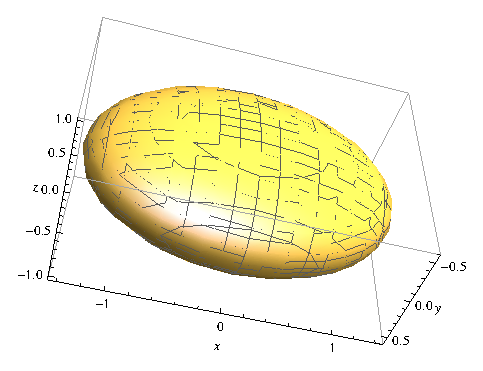
\includegraphics[scale=1]{../img/implicit_surface.eps}
\label{fig:implicit}
\caption{Implicit surface given by function $f(x,y,z) = \frac{1}{2}x^{2} + 3y^{2} + z^{2} = 1$}
\end{figure}
This representation has several advantages such as efficient checking whether a point is either
inside or outside and efficient search for an intersection with geometric primitives.


\subsection{Constructive Solid Geometry}

Known also as \emph{CSG tree}\cite{Zara2004}. This technique is used especially
in the engineering software. It allows
the user to construct objects using \emph{Boolean operators}. Objects created by using this
method can be used repeatedly in Boolean operators; the resulting object can be decomposed into a tree.
\\
\\
The leaves of the tree are typically the objects of the simple shape. However, the operators can be
theoretically applied on any objects. The set of supported primitives is given by a specific
software package.
\\
\\
Thanks to the tree structure, CSG objects come with some convenient properties. The nodes that
are higher in the tree hierarchy give us an approximation that can be used in various geometric
algorithms with no need to look for its descendants.

\subsection{Point Cloud}

A point cloud is a set of points in a three-dimensional coordinate system\cite{Zara2004}\cite{Agarwal2006}.
The set can form the surface
of an object or any other three dimensional figure. Every point is indepedent
from one another, with no information about its topology. They are often converted to polygon mesh
or triangle mesh models.

\subsection{Polygonal Mesh}

A polygonal mesh is a collection of vertices, edges and faces that defines the shape of the surface of
the object\cite{Zara2004}. Some special implementations do not contain faces. These implementations are
defined only by vertices and
edges. Moreover, some cases do not consider the topology and the object is a raw set of polygons.
Neverthless, a standard implementation is expected to contain a topology information about each vertex
and face.
\\
\\
Each face is defined by planar polygon, in special cases by \emph{convex polygon} or \emph{triagle}.
The polygonal mesh restricted to contain triangular faces only, is called \emph{triangle mesh}.
The main purpose of the restriction is the rendering simplification. In general case, face is defined
as the set of points that can contain a hole.
\\
\\
There are several techniques to represent a topology of the mesh. Each of them has its own advantages
that are reflected in an efficiency of data storage and querying the surrounding elements. Several
mesh representations are described in the next section.

\section{Polygonal Mesh}
\label{sec:polyg_mesh}
The collection can be represented in a variety of ways, the main purpose of the structure is to improve
the efficiency of the queries. On the other hand we face the limitations such as memory. In some
representations it is impossible to query the adjacent vertices of a vertex without iteration through
entire container of vertices or faces.

\subsection{Face-Vertex Mesh}
\label{sec:face-vertex}

The simplest representation that contains any information about topology of the polygonal
mesh. A mesh is represented by a container of vertices and the container of sets of vertices that
form faces\cite{Zara2004}. The face is represented by at least 3 vertices or more vertices that have to be
coplanar.\\

\begin{figure}[h]

\begin{minipage}[hb]{0.65\linewidth}
\centering
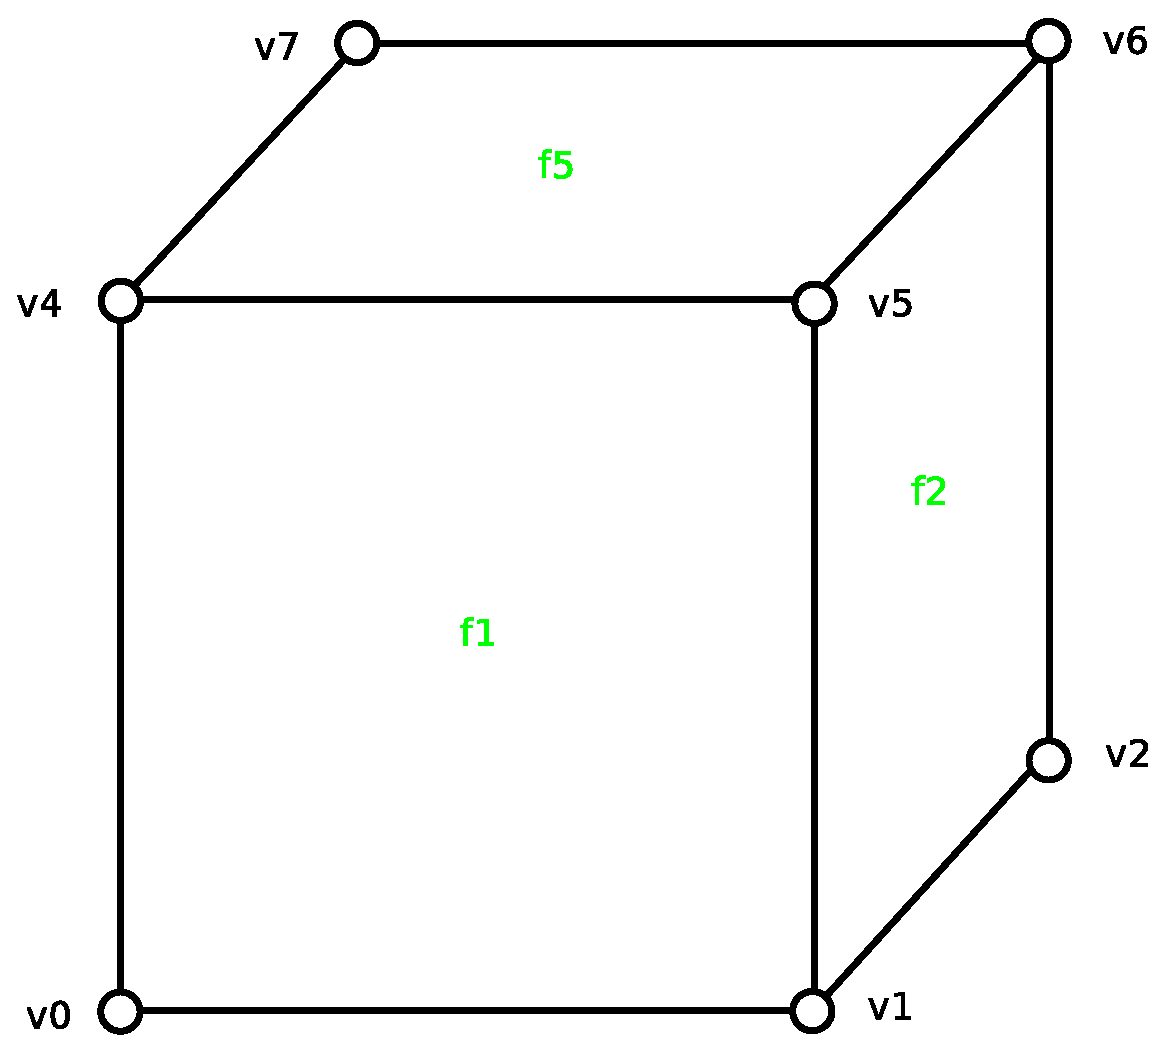
\includegraphics[width=0.6\linewidth]{../img/fv_rep_mesh.eps}
\label{fig:figure1}
\end{minipage}
\hspace{0.5cm}
\begin{minipage}[hb]{0.25\linewidth}
\centering
\begin{tabular}{|c|c|}
\hline
\textsf{v0 v1 v5 v4} & \textsf{f1}\\
\hline
\textsf{v1 v2 v6 v5} & \textsf{f2}\\
\hline
\textsf{v4 v5 v6 v7} & \textsf{f5}\\
\hline
\end{tabular}
\label{fig:fv_mesh}
\end{minipage}

\caption{face-vertex mesh representation}
\end{figure}

The set that forms the faces must be ordered. The preceding and following vertex in order must be 
adjacent to
the vertex. If the structure is not extended by face-normal-attribute, the vertices have to be in 
clockwise/counter-clockwise order from the view of face normal. Whether the order is clockwise or counter-clockwise
depends on the implementation of the mesh.

\subsection{Winged-Edge mesh}

The representation described above contains no direct information about adjacency of faces. 
In order to determine the adjacency of any two faces or vertices in constant complexity, we
can build a structure that requires an extra storage. The winged edge structure\cite{Baumgart1972}
provides information
capable of determining edges that belong to a vertex. It also provides information which allows us
to determine the surrounding edges from the given face;
in case of a triangle mesh, it returns the triplet of edges.
Finally, the structure is named \emph{winged-edge} because of its
capabilty to get a face pair (wings) from
a given edge.

\begin{figure}[!htbp]
\label{fig:winged_edge_mesh}

\begin{minipage}[!htbp]{0.65\linewidth}
\centering
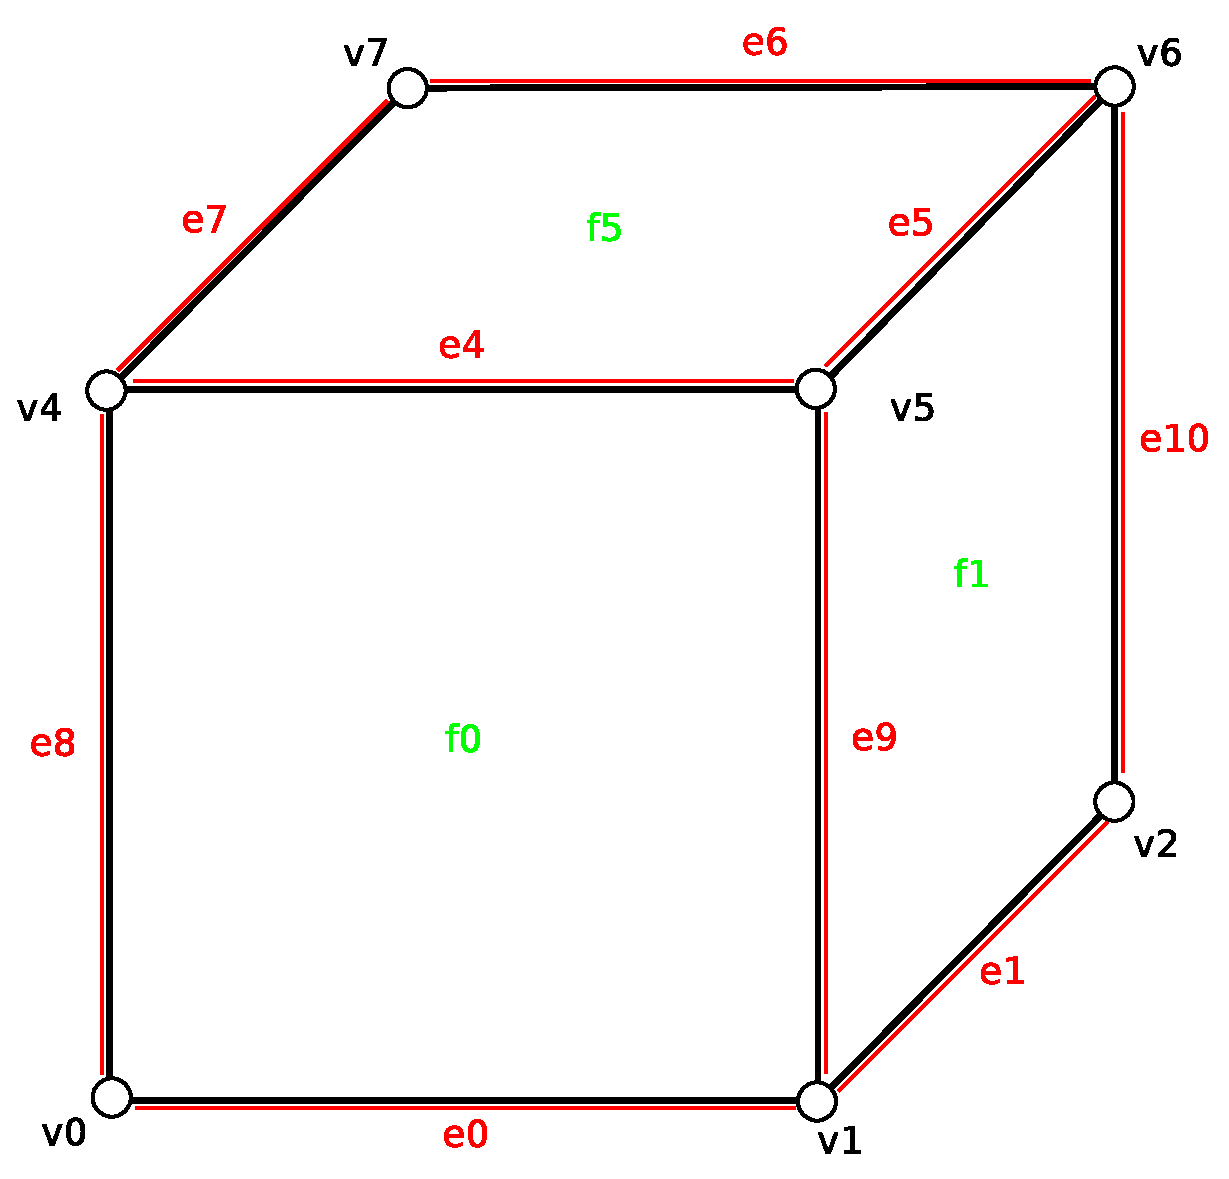
\includegraphics[width=0.6\linewidth]{../img/we_rep_mesh.eps}
\label{fig:figure1}
\end{minipage}
\hspace{0.5cm}
\begin{minipage}[!htbp]{0.25\linewidth}
\centering

\emph{Face list}
\vspace{1mm}

\begin{tabular}{|c|c|}
\hline
\textsf{f0} & \textsf{e0 e9 e4 e8}\\
\hline
\textsf{f1} & \textsf{e1 e10 e5 e9}\\
\hline
\textsf{f5} & \textsf{e4 e5 e6 e7}\\
\hline
\end{tabular}

\vspace{10mm}
\emph{Edge list}
\vspace{1mm}

\begin{tabular}{|c|c|c|}
\hline
\textsf{e0} & \textsf{f0 f4} & \textsf{v0 v1}\\
\hline
\textsf{e1} & \textsf{f1 f4} & \textsf{v1 v2}\\
\hline
\textsf{e4} & \textsf{f0 f5} & \textsf{v4 v5}\\
\hline
\textsf{e5} & \textsf{f1 f5} & \textsf{v5 v6}\\
\hline
\textsf{e6} & \textsf{f2 f5} & \textsf{v6 v7}\\
\hline
\textsf{e7} & \textsf{f3 f5} & \textsf{v7 v8}\\
\hline
\textsf{e8} & \textsf{f0 f3} & \textsf{v4 v0}\\
\hline
\textsf{e9} & \textsf{f1 f0} & \textsf{v5 v1}\\
\hline
\textsf{e10} & \textsf{f2 f1} & \textsf{v6 v2}\\
\hline
\end{tabular}

\label{fig:we_mesh}
\end{minipage}

\caption{Winged-edge mesh}
\end{figure}

%On the example shown above there are occured several uncertainities.
Several uncertainities occured in the above-mentioned examples.

\begin{itemize}
\item Let us take edge \textsf{e9}. In the pair of faces, which of faces \textsf{f0} and 
\textsf{f1} should be considered as the \emph{first} and which as the \emph{second}?

\item Which of vertices \textsf{v1} and \textsf{v5} should be considered as 
the \emph{first} and which as the \emph{second} in the pair that forms the edge \textsf{e9}?
\end{itemize}

One of possible solutions is to split the edge element into two \emph{half-edges}.
The structure using, or rather based on this representation, is described in the next
paragraph.

\subsection{Half-Edge mesh}

The half-edge data structure is the structure capable of maintaining the incidence
information of vertices, edges and faces\cite{Botsch2006}. Each edge is decomposed in two half-edges
with opposite orientations.
\\

The structure contains the set of following information
\begin{itemize}
\item a vertex that is the half-edge pointing to
\item a face that the half-edge belongs to
\item the next half-edge in order that forms a face that half-edge belongs to
\item (optional) the previous half-edge in the same order
\item opposite half-edge
\end{itemize}

\begin{figure}[h]

\begin{minipage}[hb]{0.65\linewidth}
\centering
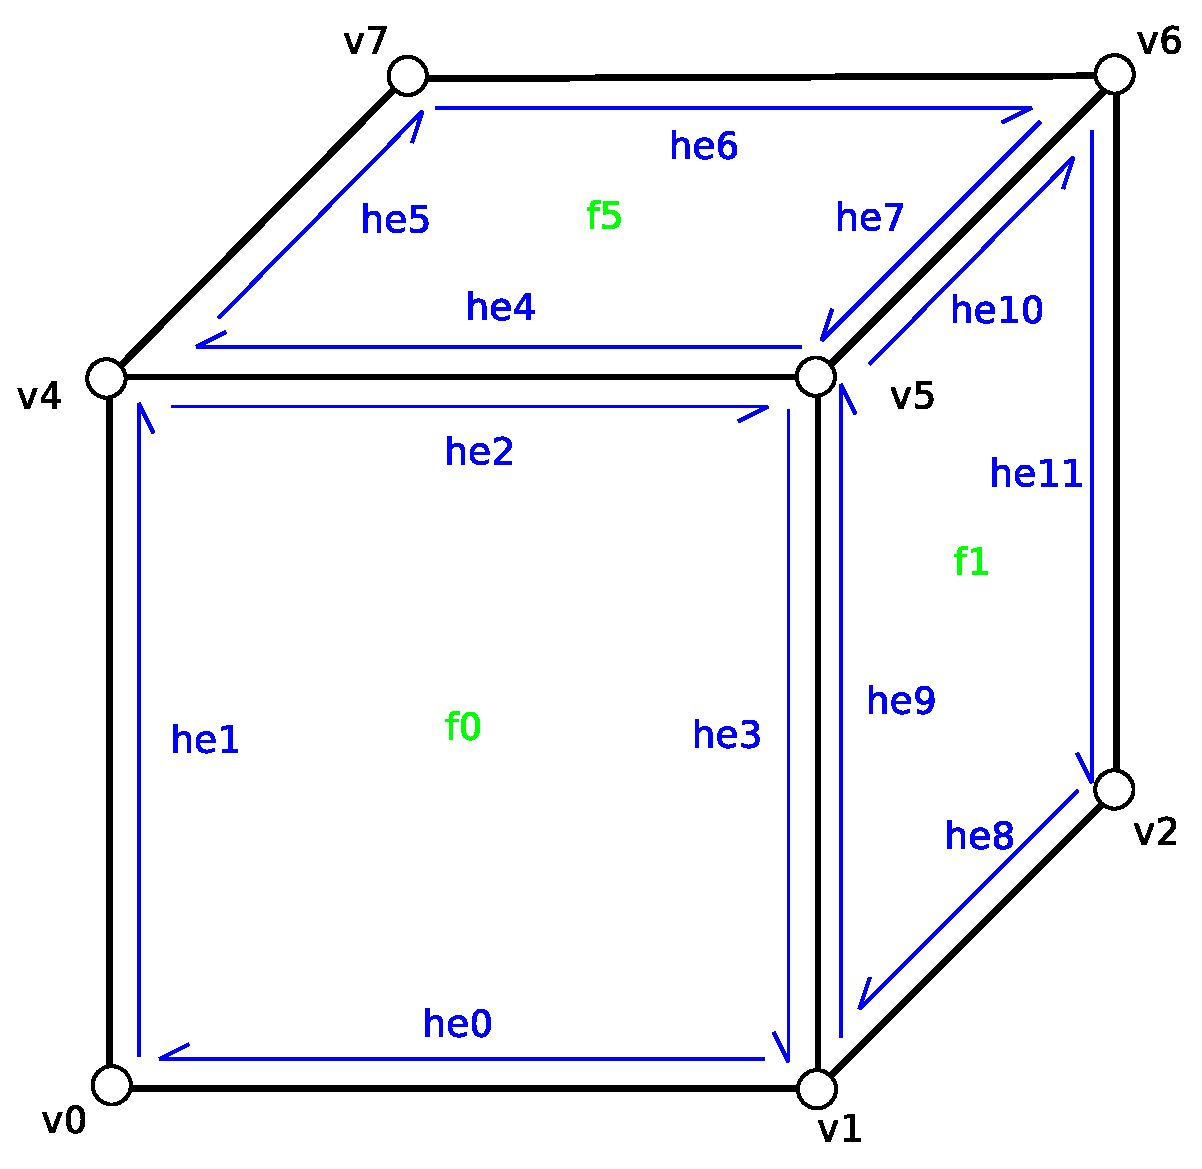
\includegraphics[width=0.6\linewidth]{../img/he_rep_mesh.eps}
\label{fig:figure1}
\end{minipage}
\hspace{0.5cm}
\begin{minipage}[hb]{0.25\linewidth}
\centering
\emph{Half-edge list}
\vspace{1mm}

\begin{tabular}{|c|c|c|c|}
\hline
\textsf{he0} & \textsf{f0} & \textsf{v0} & \textsf{he1}\\
\hline
\textsf{he1} & \textsf{f0} & \textsf{v4} & \textsf{he2}\\
\hline
\textsf{he2} & \textsf{f0} & \textsf{v5} & \textsf{he3}\\
\hline
\textsf{he3} & \textsf{f0} & \textsf{v1} & \textsf{he0}\\
\hline

\hline
\textsf{he8} & \textsf{f1} & \textsf{v1} & \textsf{he9}\\
\hline
\textsf{he9} & \textsf{f1} & \textsf{v5} & \textsf{he10}\\
\hline
\textsf{he10} & \textsf{f1} & \textsf{v6} & \textsf{he11}\\
\hline
\textsf{he11} & \textsf{f1} & \textsf{v2} & \textsf{he8}\\
\hline

\hline
\textsf{he4} & \textsf{f5} & \textsf{v4} & \textsf{he5}\\
\hline
\textsf{he5} & \textsf{f5} & \textsf{v7} & \textsf{he6}\\
\hline
\textsf{he6} & \textsf{f5} & \textsf{v6} & \textsf{he7}\\
\hline
\textsf{he7} & \textsf{f5} & \textsf{v5} & \textsf{he4}\\
\hline
\end{tabular}
\label{fig:he_mesh}
\end{minipage}

\caption{Half-edge mesh representation}

\end{figure}

\chapter{Operations and algorithms}

Our aim in this chapter is to describe algorithms over 3D data structures. In each description of
algorithm there is a short paragraph that summarizes required operations for running the algorithm.
It is later used in hierarchical implementation of the algorithms.

\section{Converting between representations}

In this section is introduced some algorithms that convert from one representation to another. Each 
representation has it's own capability.

\subsection{Delaunay triangulation}

Let $P$ be a set of points in the $d$-dimensional Euclidean space.
Delanuay triangulation is triangulation such that no point $p \in P$ is inside the circum-hypersphere
of any simplex in $DT(P)$. For better imagination, in case of $2$-dimensional space no point
structure is inside the circumcircle of any triangle of resulting structure.

\subsection{Marching cubes}

Marching cubes algorithm converts from a grid representation to a mesh. It iterates through
all grid elements and build a new polygonial mesh. For an each element (can be considered as \emph{cube}.
In some cases, it can be cuboid or even parallelepiped.)
it determines whether the corners are inside or outside object. The algorithm considers only the elements
those contains both categories of points; rest of them are ignored. As each element has 8 corners,
each of them can be determined either as inside or outside object, in result element can possibly
have one of $2^8 = 256$ configurations. However, some configurations can fit to another after rotation
or reflective simmetry or sign changed case.\\


\begin{figure}[ht]
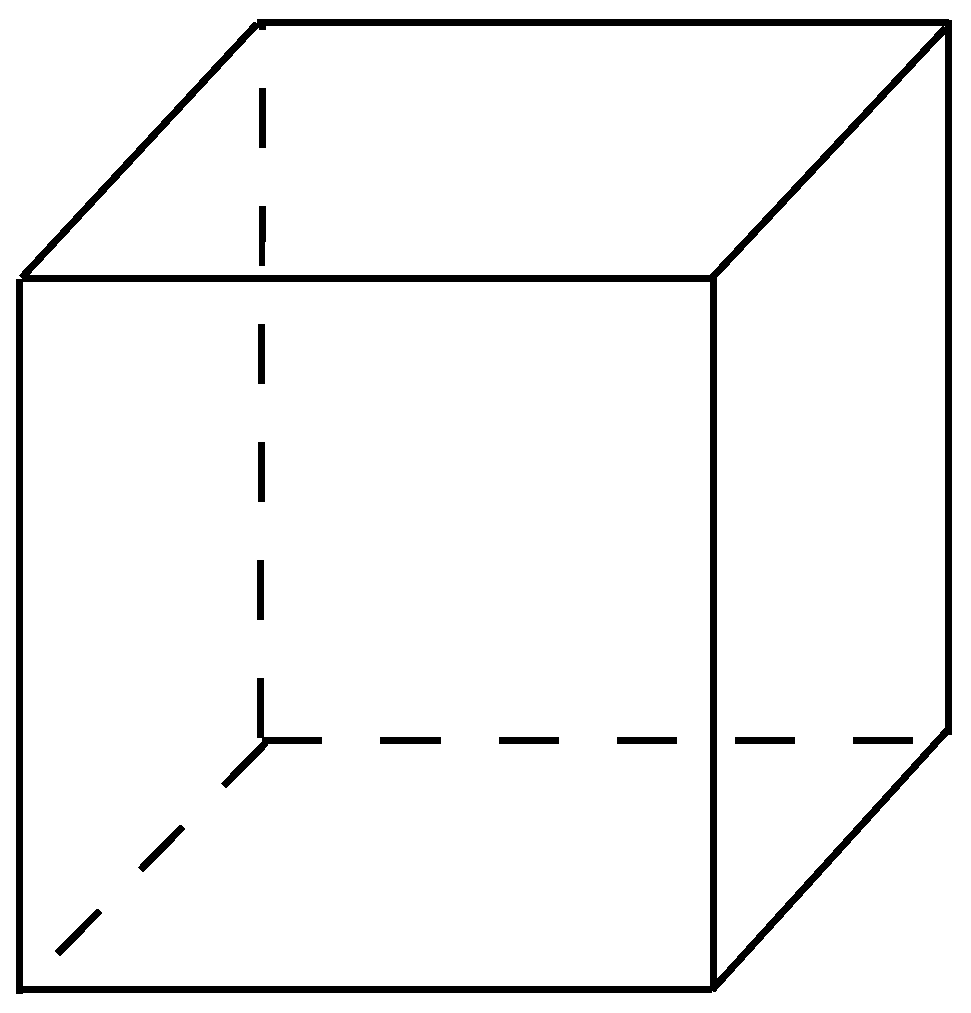
\includegraphics[scale=0.15]{../img/mar_cub_case0.eps}
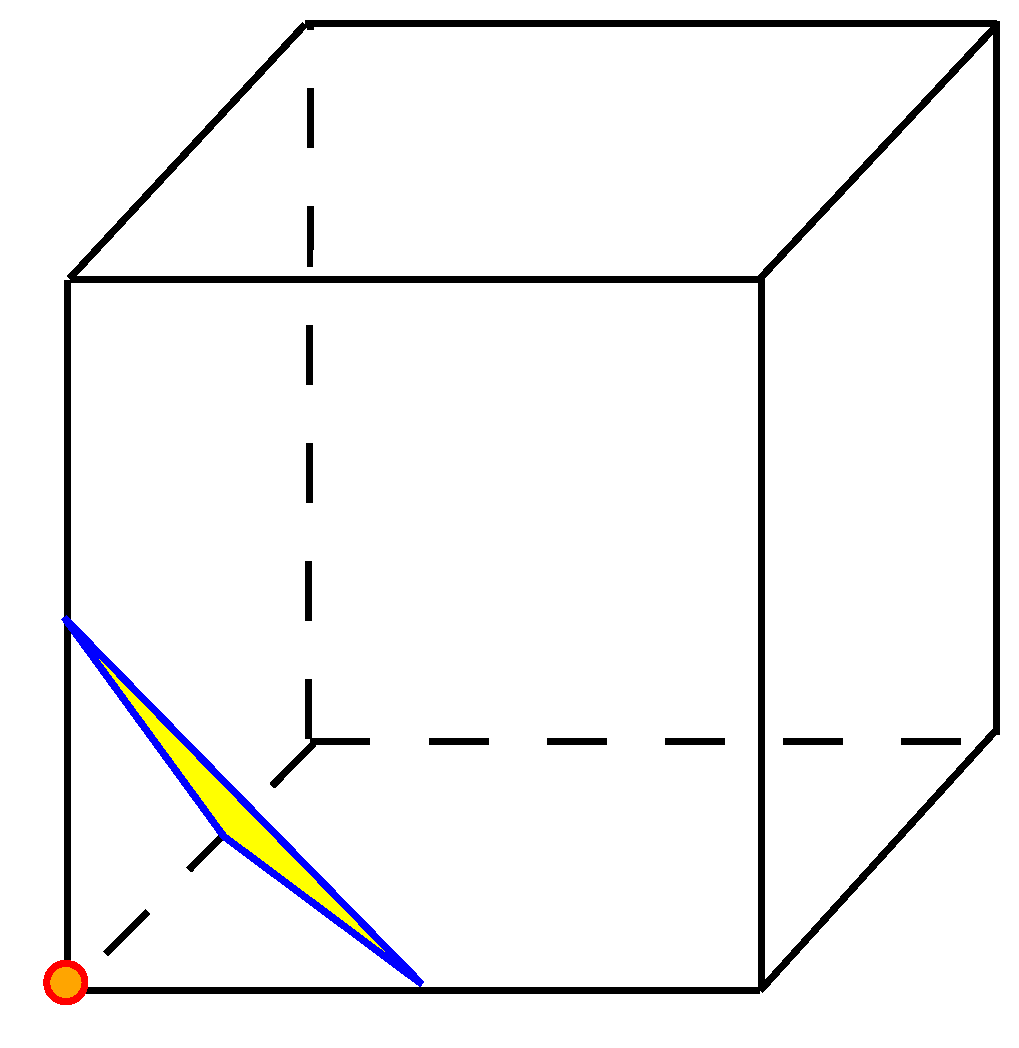
\includegraphics[scale=0.15]{../img/mar_cub_case1.eps}
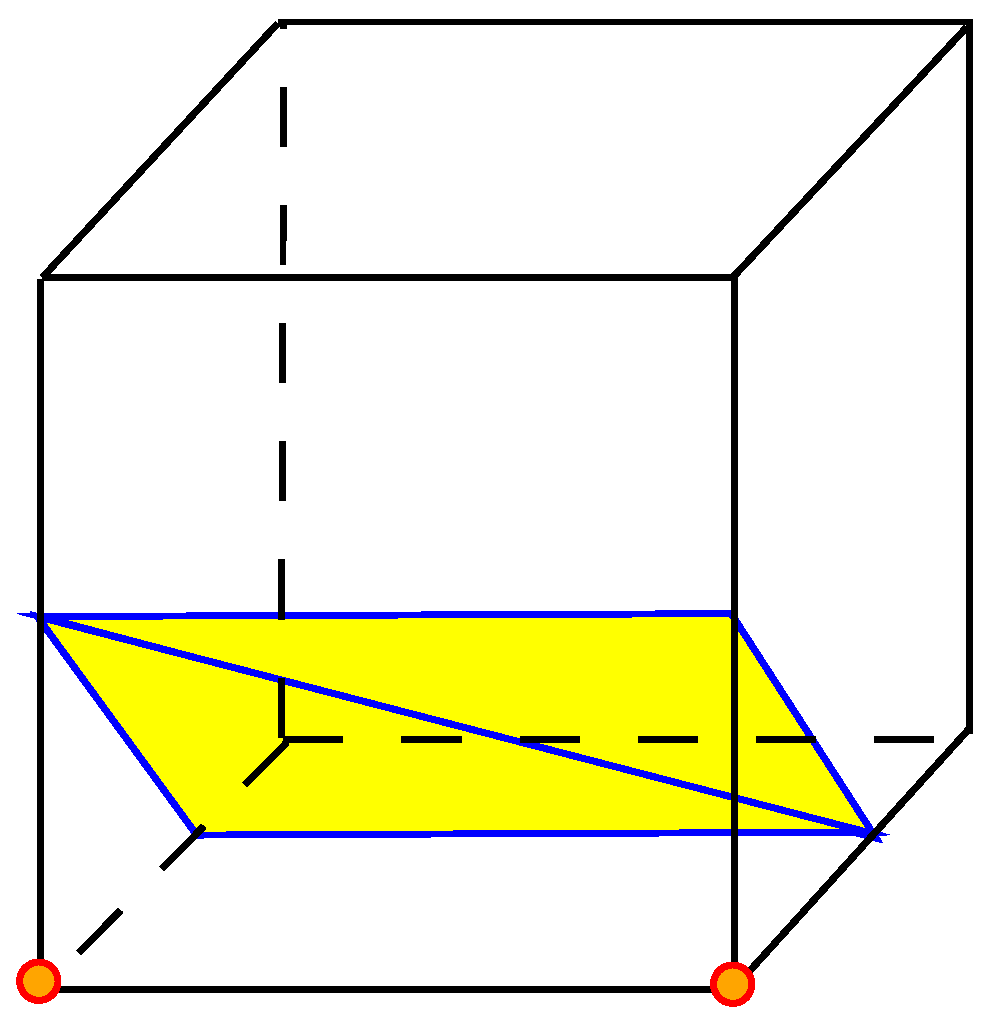
\includegraphics[scale=0.15]{../img/mar_cub_case2.eps}
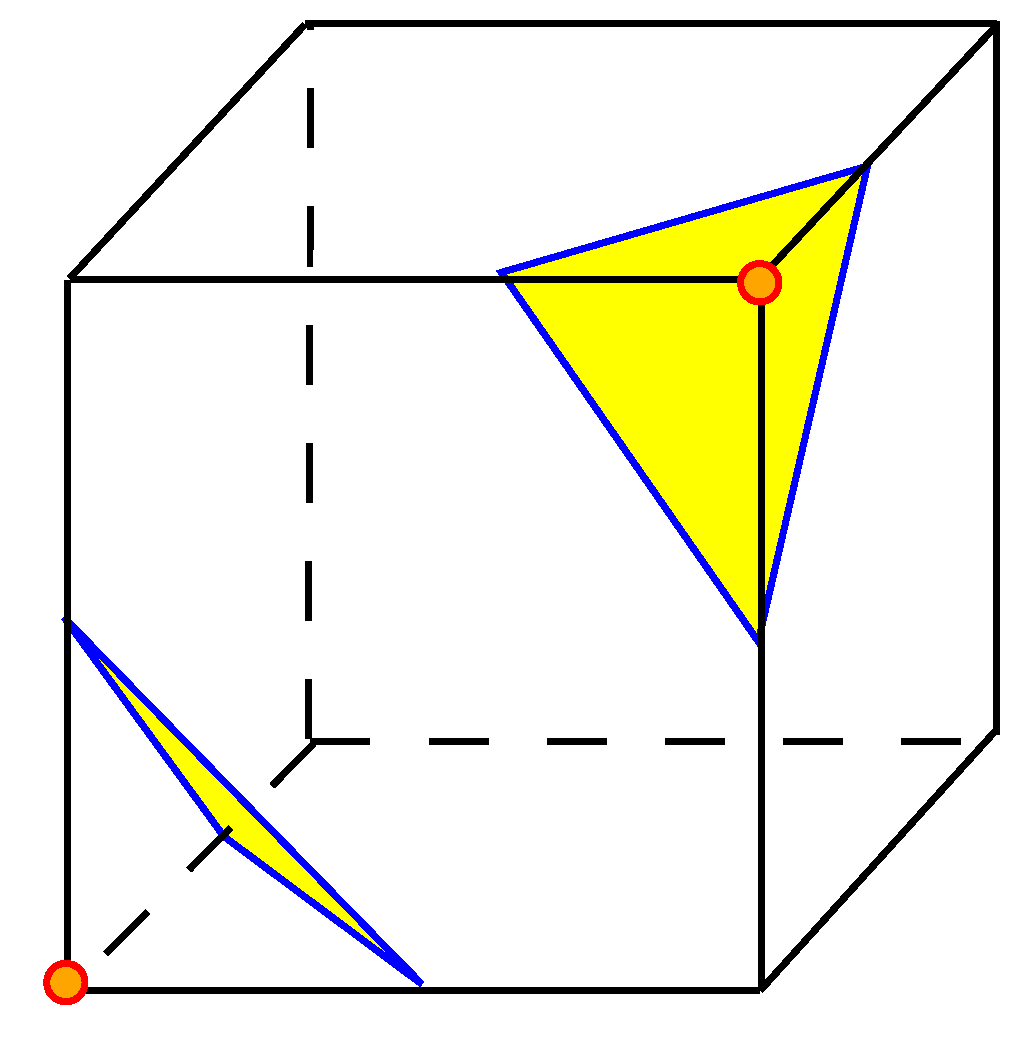
\includegraphics[scale=0.15]{../img/mar_cub_case3.eps}
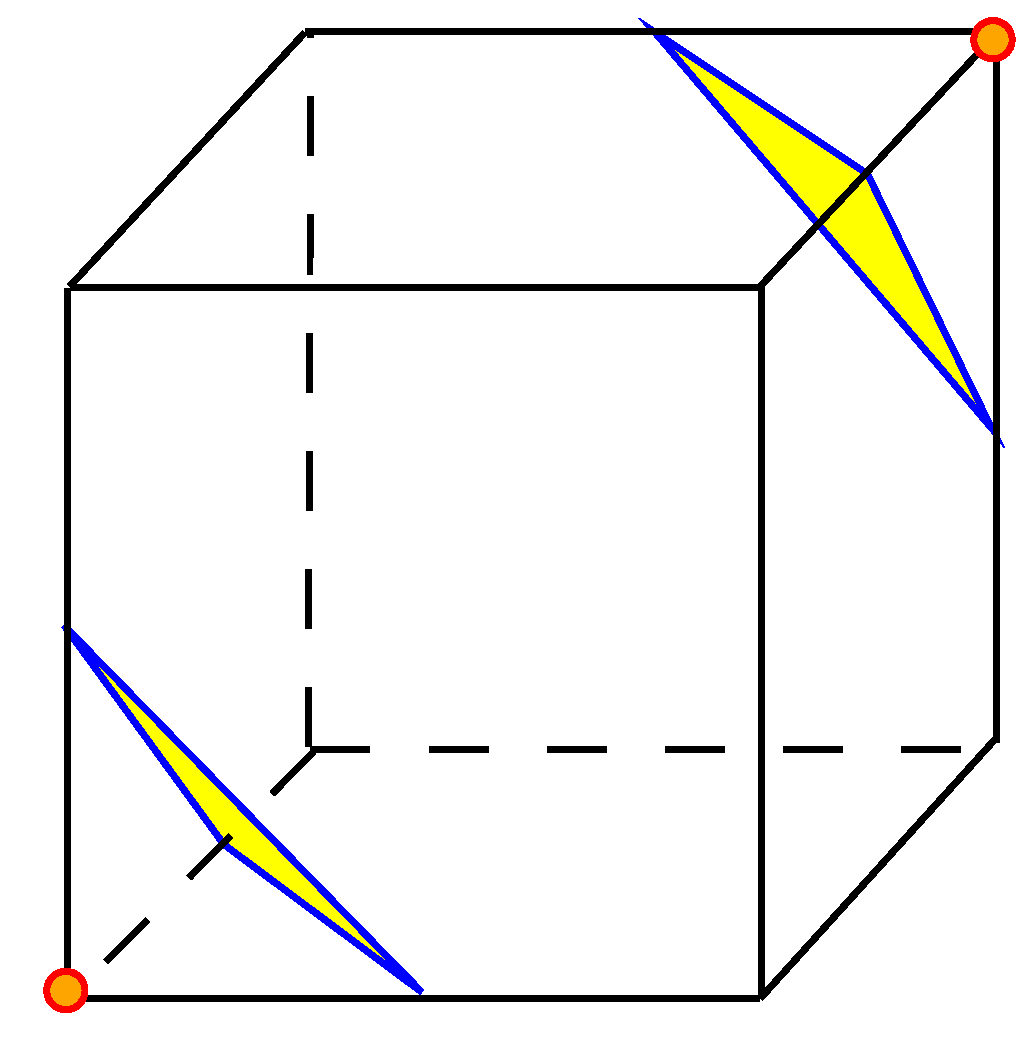
\includegraphics[scale=0.15]{../img/mar_cub_case4.eps}
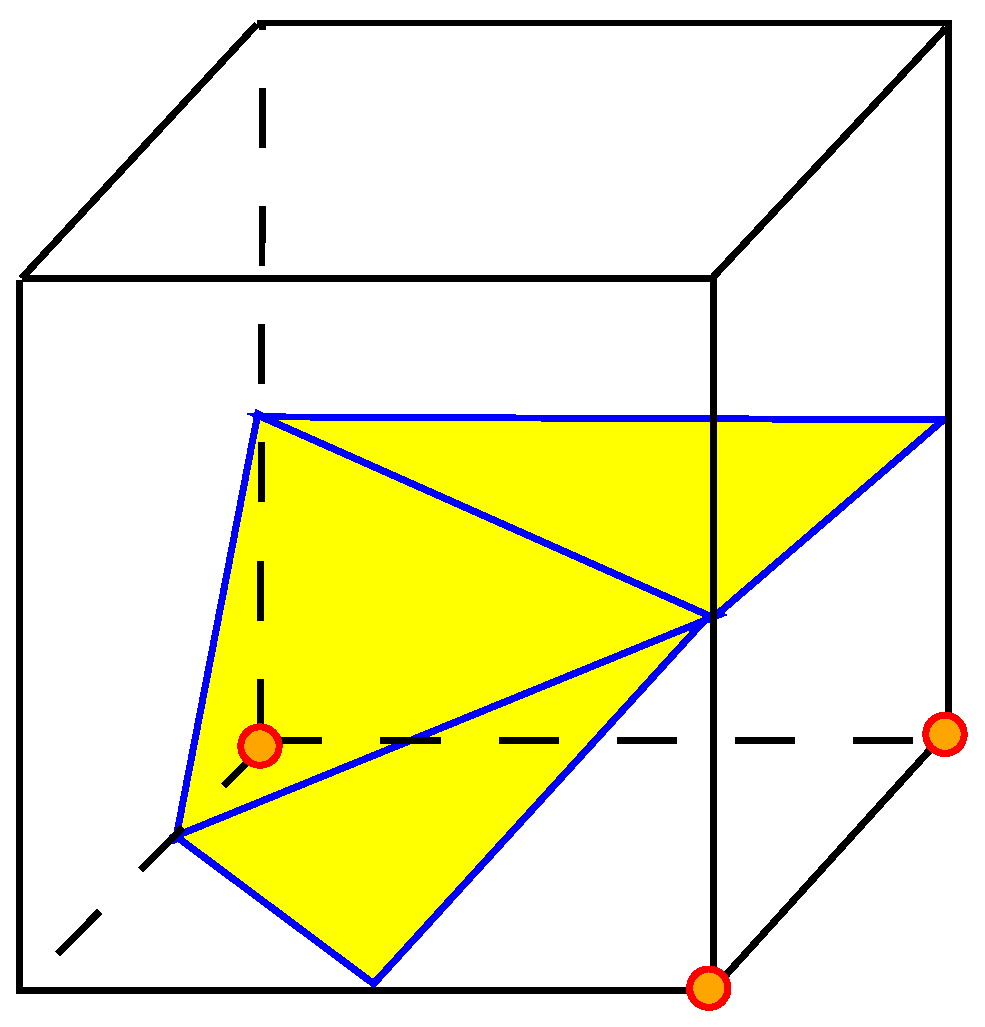
\includegraphics[scale=0.15]{../img/mar_cub_case5.eps}
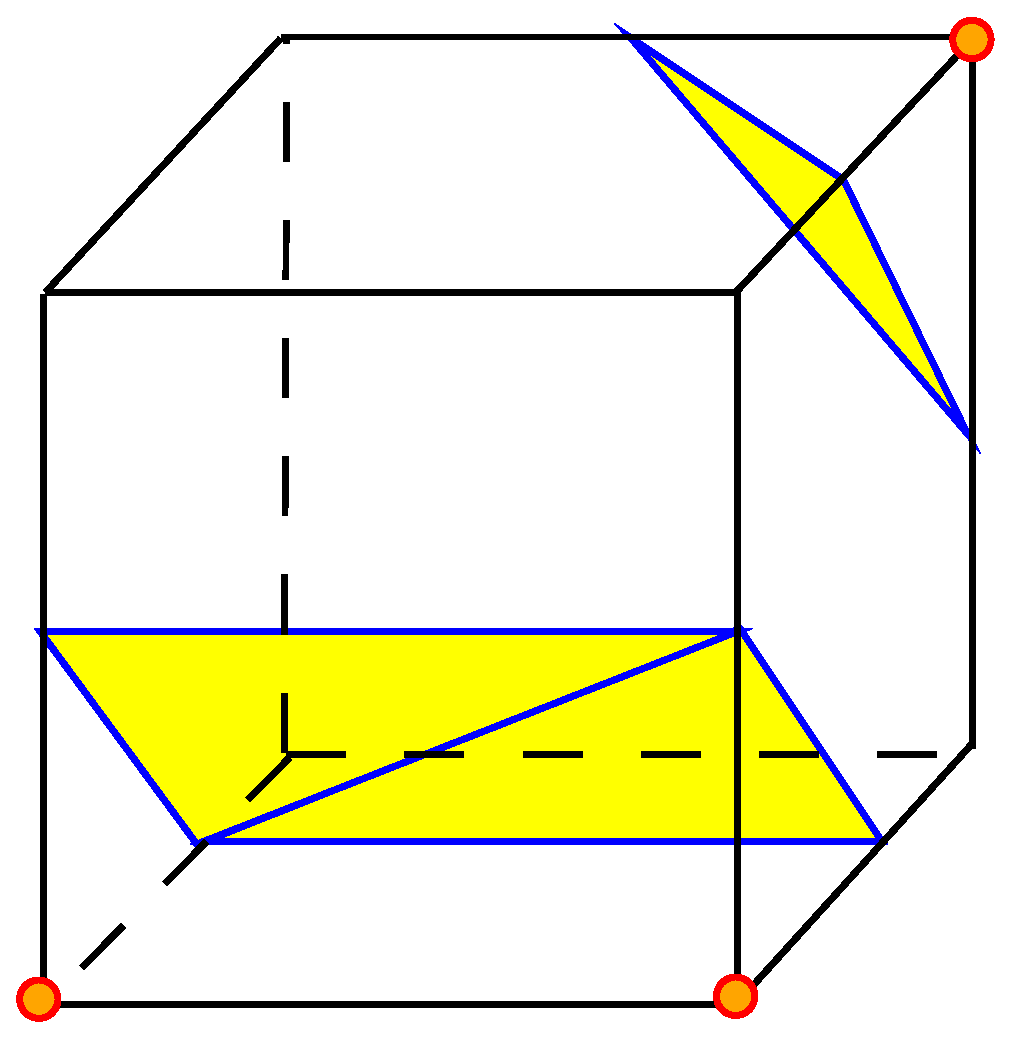
\includegraphics[scale=0.15]{../img/mar_cub_case6.eps}
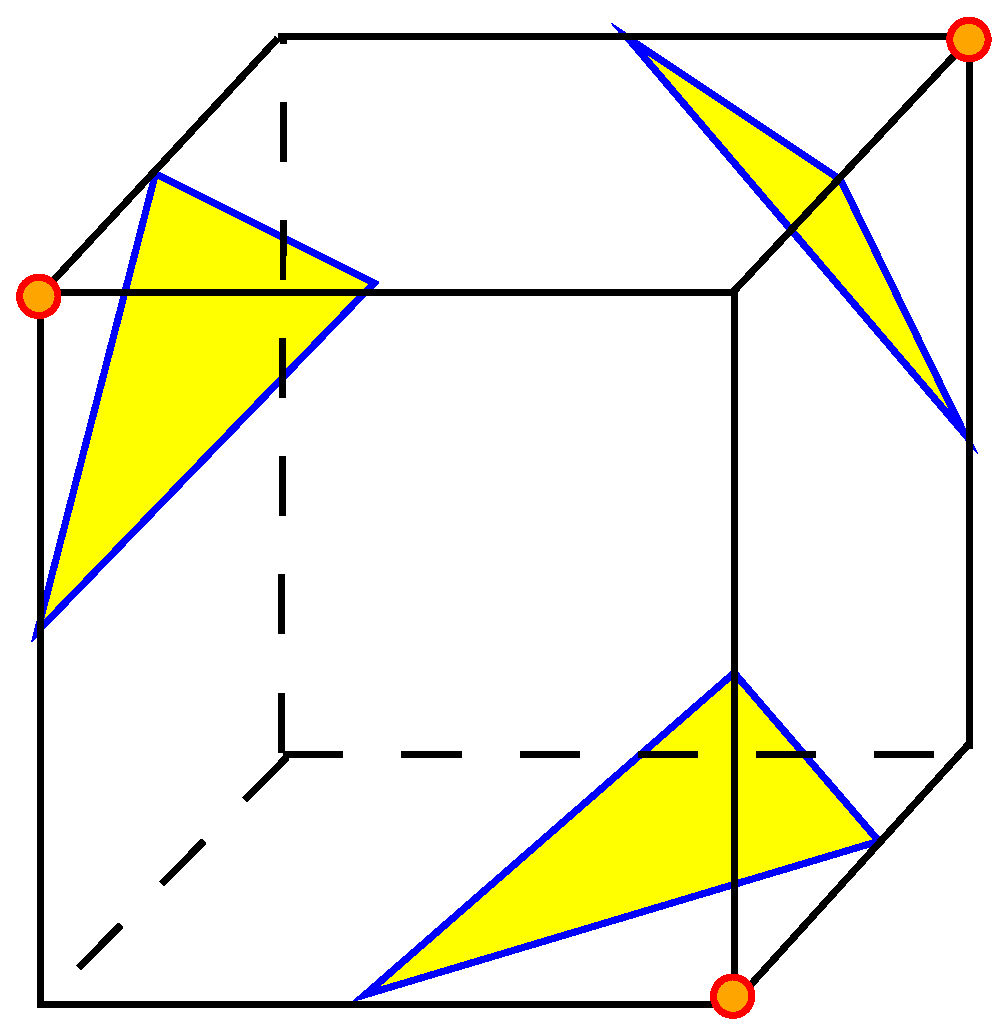
\includegraphics[scale=0.15]{../img/mar_cub_case7.eps}
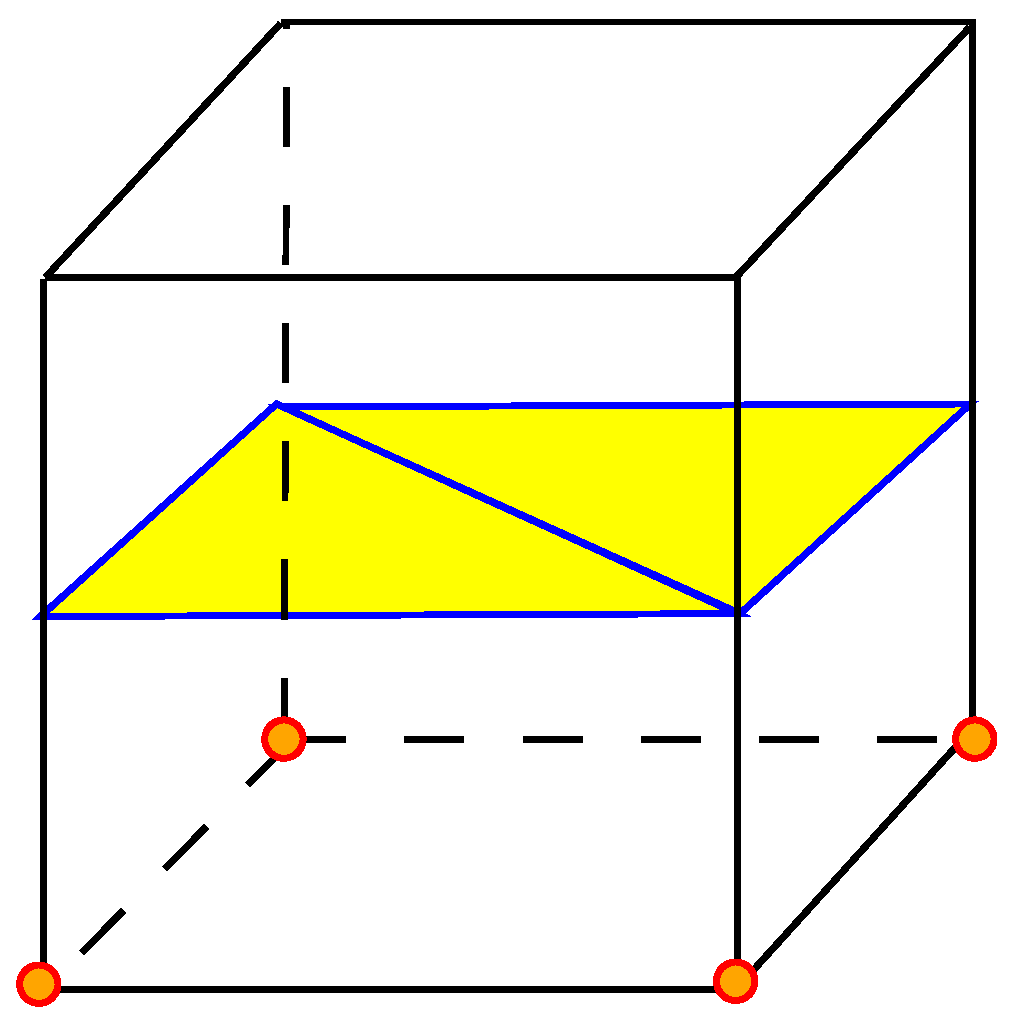
\includegraphics[scale=0.15]{../img/mar_cub_case8.eps}
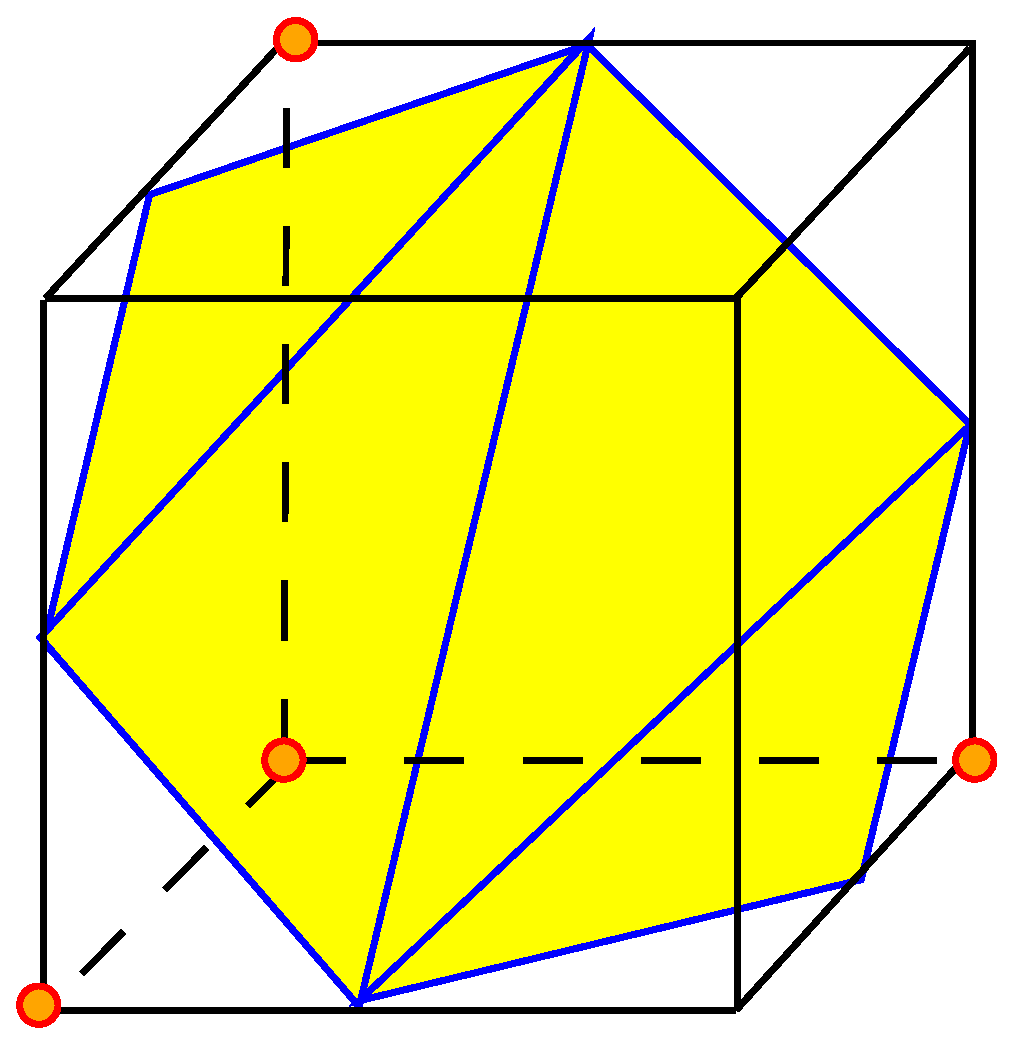
\includegraphics[scale=0.15]{../img/mar_cub_case9.eps}
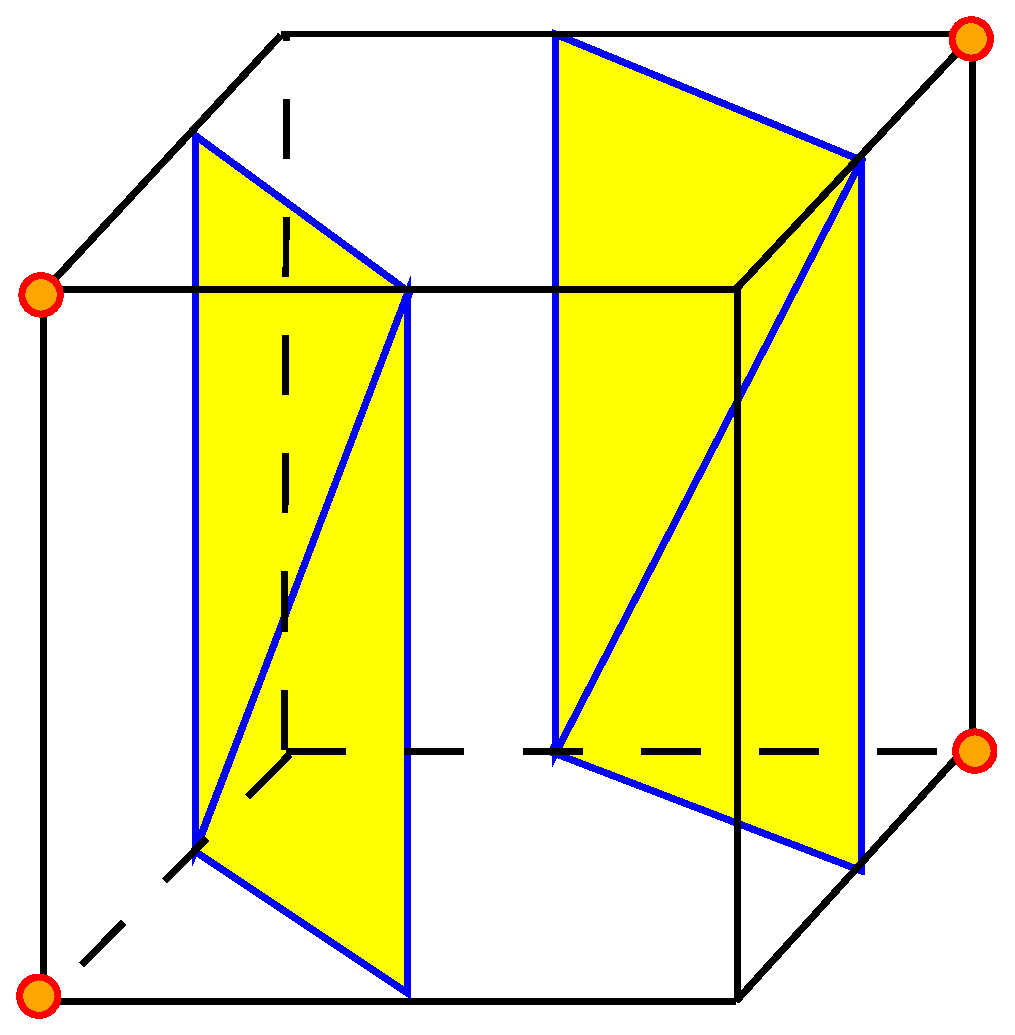
\includegraphics[scale=0.15]{../img/mar_cub_case10.eps}
\hspace{1mm}
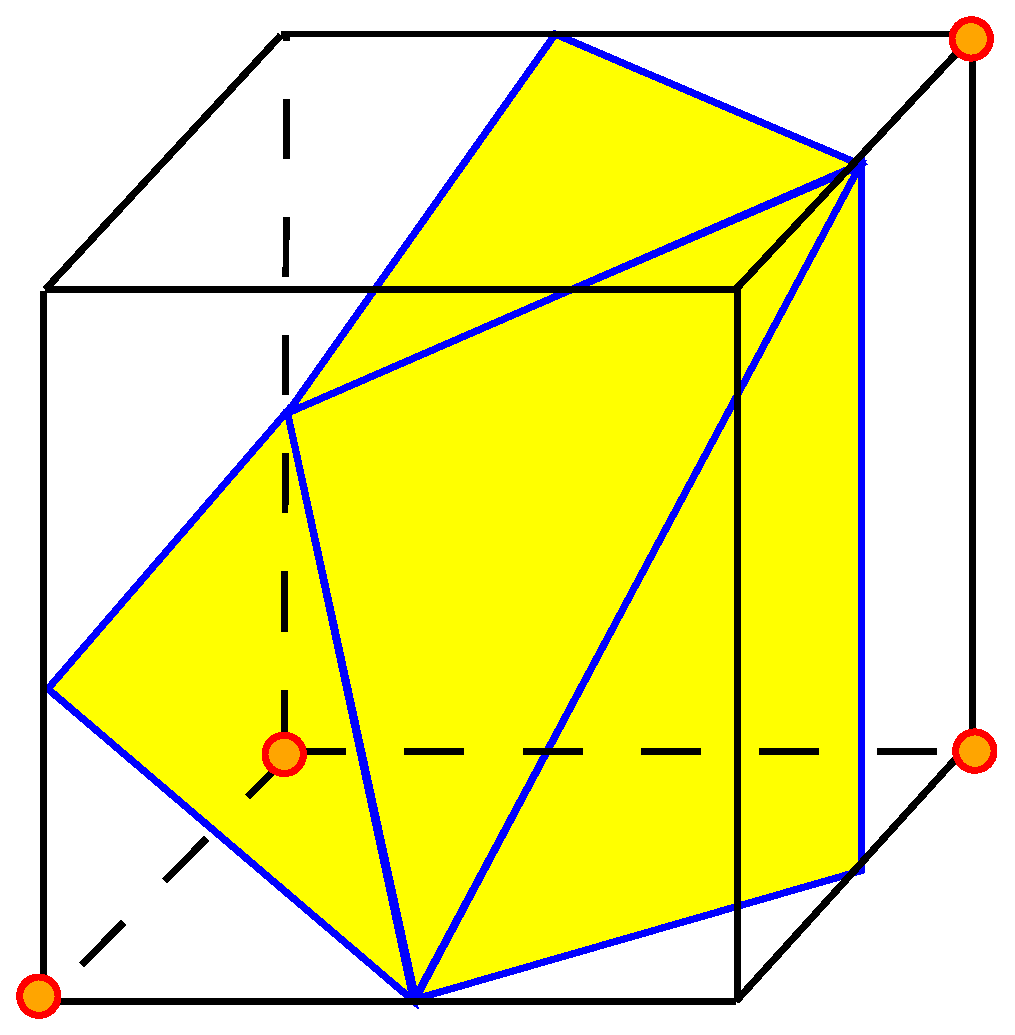
\includegraphics[scale=0.15]{../img/mar_cub_case11.eps}
\hspace{2mm}
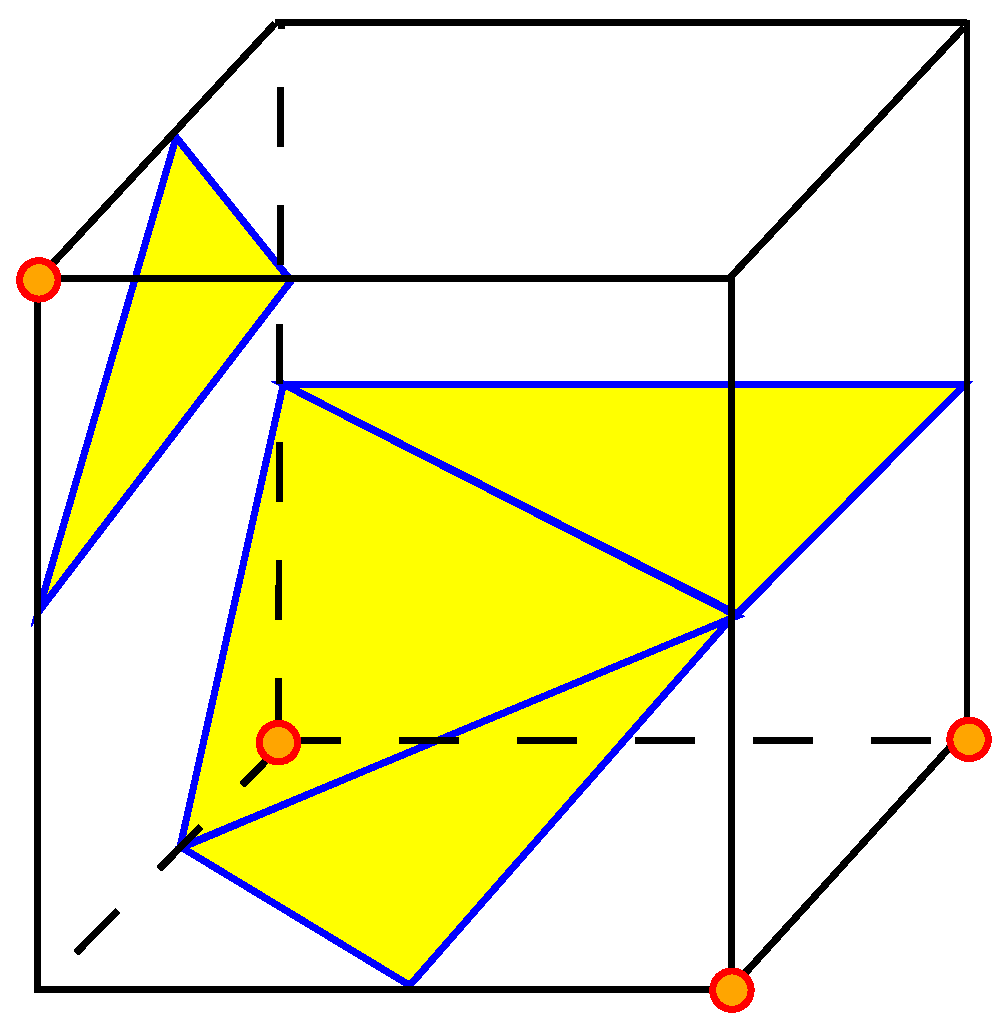
\includegraphics[scale=0.15]{../img/mar_cub_case12.eps}
\hspace{2mm}
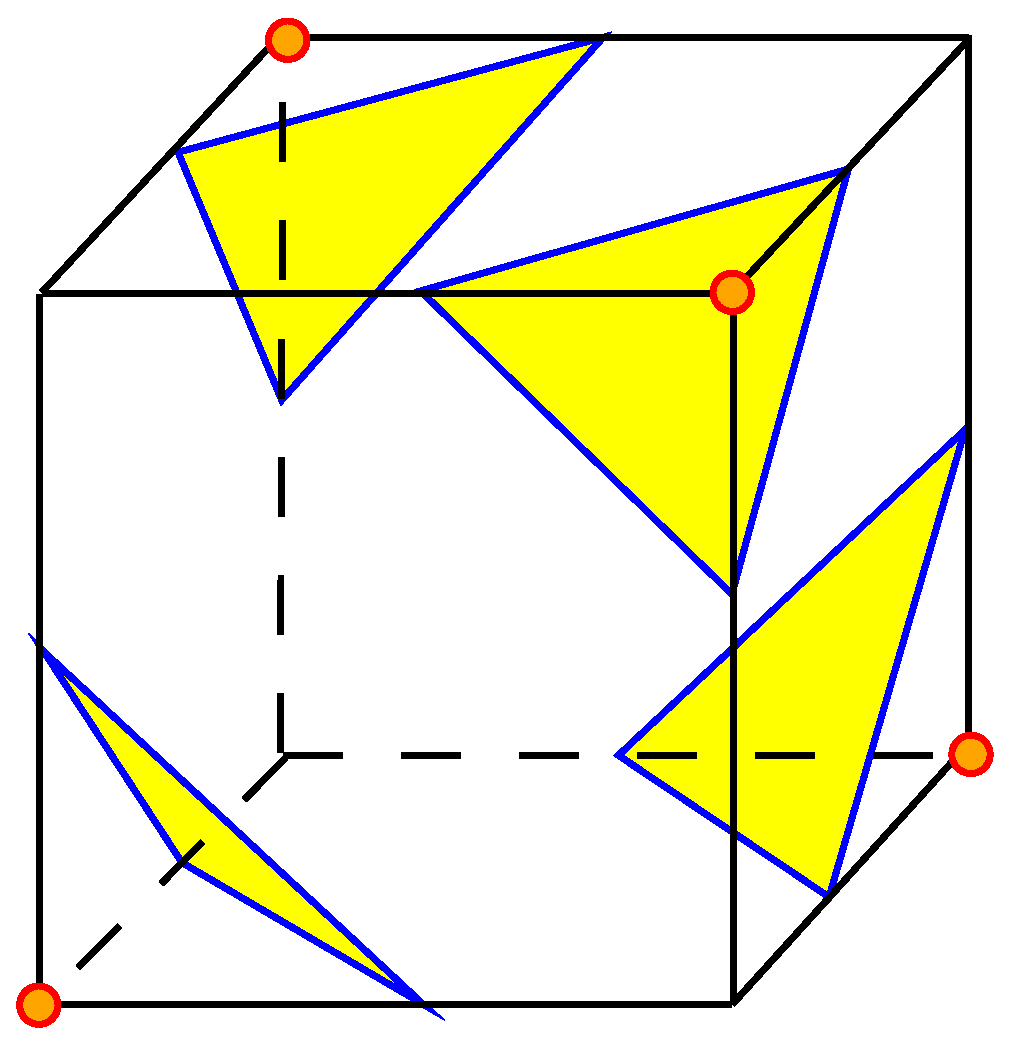
\includegraphics[scale=0.15]{../img/mar_cub_case13.eps}
\hspace{3mm}
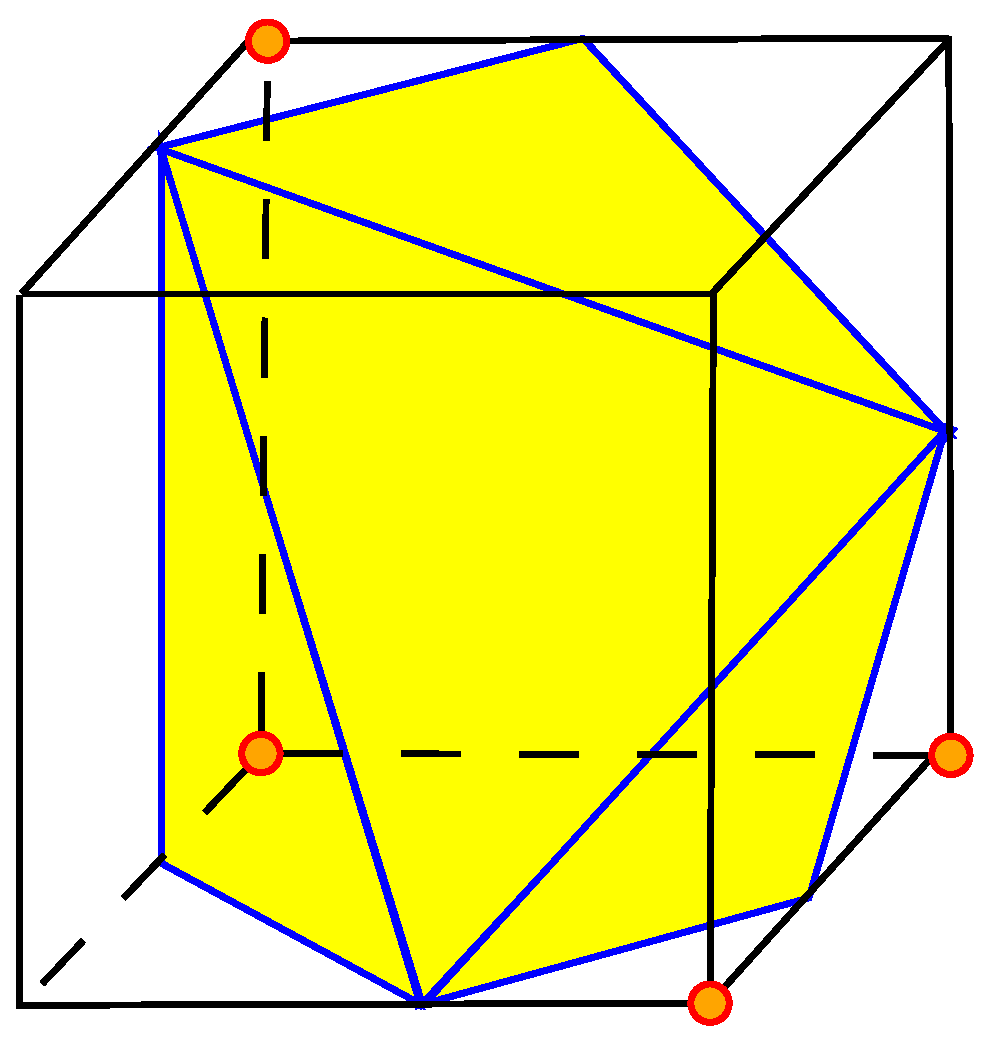
\includegraphics[scale=0.15]{../img/mar_cub_case14.eps}
\caption{The 15 cases of marching cubes algorithm. The corners that are evaluated as inside of the object
are labeled with red. The yellow triangles represent faces to be added to mesh.}
\label{fig:mc_cases}
\end{figure}

Finaly, all of them can be reduced to $15$ unique cases. The main idea of this algorithm is to
place a set of faces for each cube in order to create a polygonal mesh with a corresponding shape.
In the other words, each configuration refers to the configuration of new faces to be added to a mesh.
However we know two adjoining elements share 4 corners, resulting faces are continuous certainly.
If corners contain any other information except from inside/out information, the position of 
the faces in the mesh can be refined. Usually it contains the information about a color or
a distance from point to surface. In that case, placing or any other processing of
the face is based on linear interpolation corner values.\\
\\

\begin{figure}[ht]
\centering
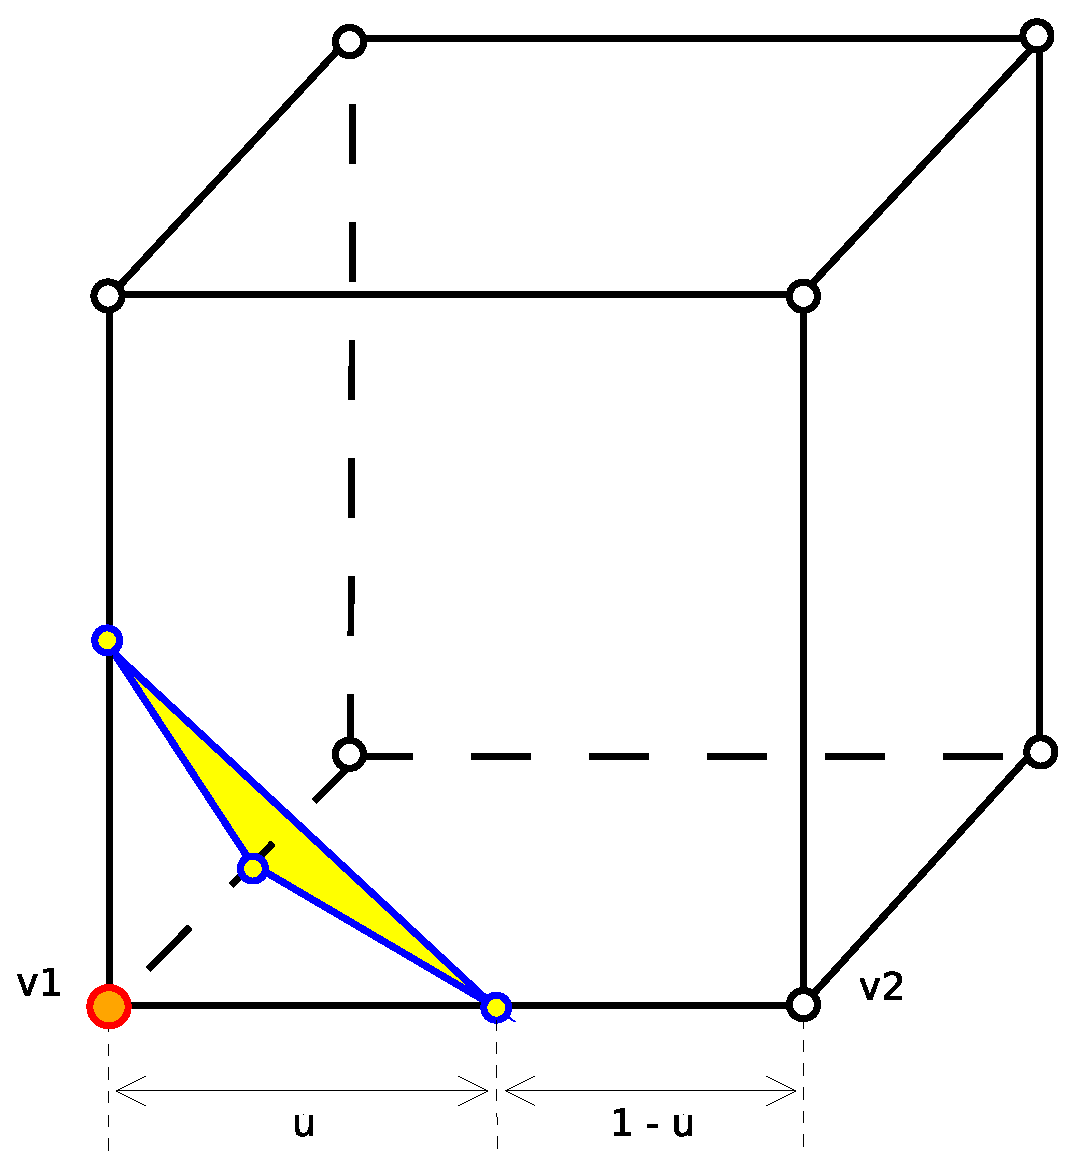
\includegraphics[scale=0.35]{../img/marc_cub_inter.eps}
\label{fig:mc_interpolation}
\end{figure}

Let $v1$ and $v2$ be the values that represents a distance from a surface to the corner.
Thus we can calculate the value of coefficient $u$ from following equation.

\begin{equation}
u = \frac{v1}{v1-v2}
\end{equation}

%This algorithm requires the capability of voxel map (or any other grid-aligned data structure) to
%determine corners configurations of arbitrary voxel (or proper element of representation). In the other
%hand, algorithm needs standard operations for creating faces and vertices of mesh.

\subsection{Voxelization}

In 2D, known as \emph{rasterization}. The algorithm that constructs an initially empty 3D grid and fill 
the
grid elements that indicates whether the element is inside the object. There is a several techniques
to represent a boundary element. The simpliest one is to set the boundary element as completely filled, 
thus we have a voxel map of values $0$ and $1$.\\

Algorithm can be divided to two phases: The first phase voxelizes the faces of triangle mesh and the
second one fill the created object. Admittedly, before the filling the object algorithm has to check,
whether the mesh forms an enclosed surface. If it does not form an enclosed surface, the second phase of
algorithm is omitted.\\

First phase voxelizes faces one by one. Each face is processed similarly like in the triangle 
rasterization in 2D.
First, algorithm voxelizes the boundary edges and then runs floodfill over the face. The filling
technique of the face is is processed by the line filling algorithm in following steps. 

\begin{figure}
\centering
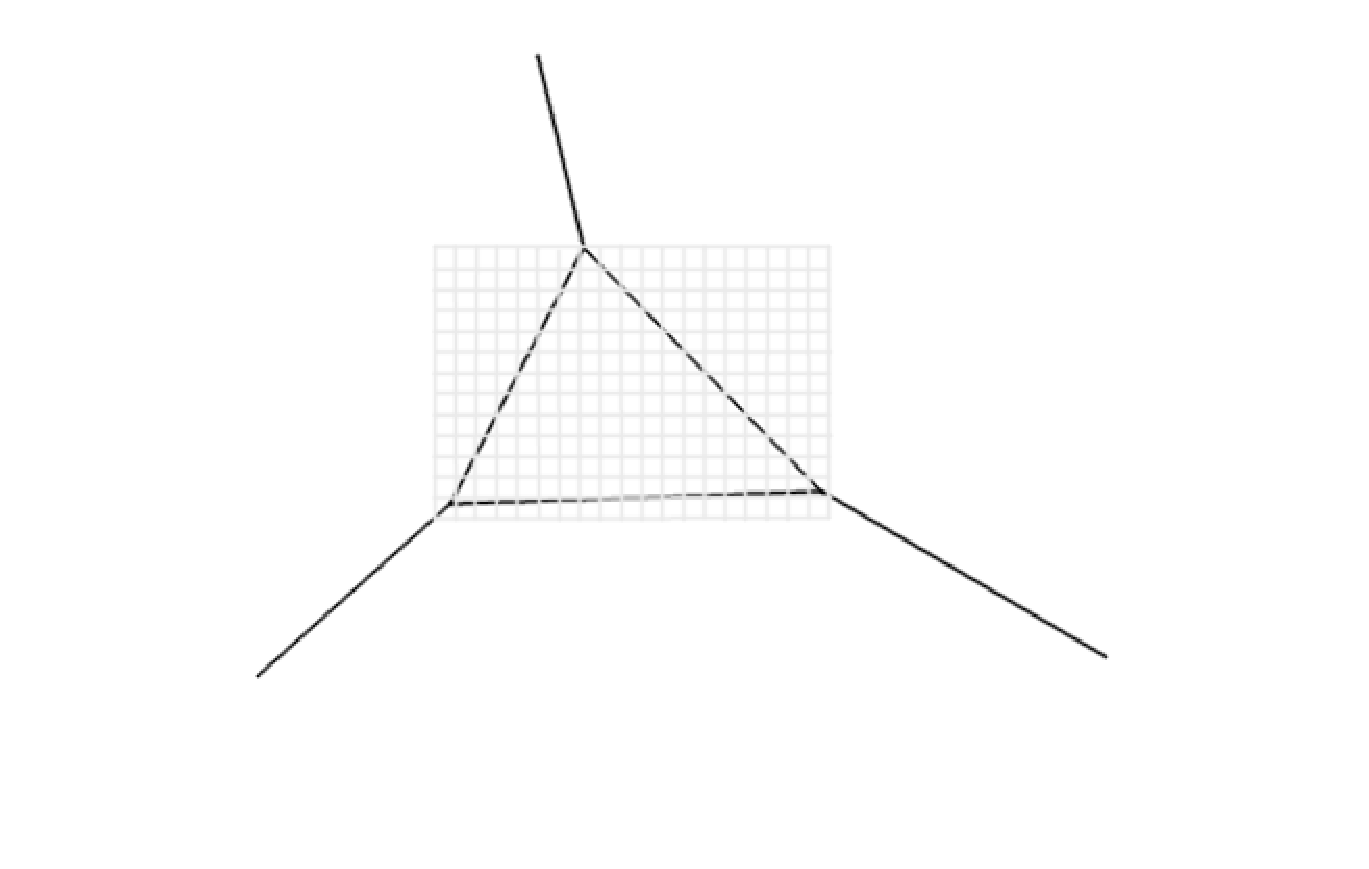
\includegraphics[scale=0.25]{../img/voxelize_1.eps}
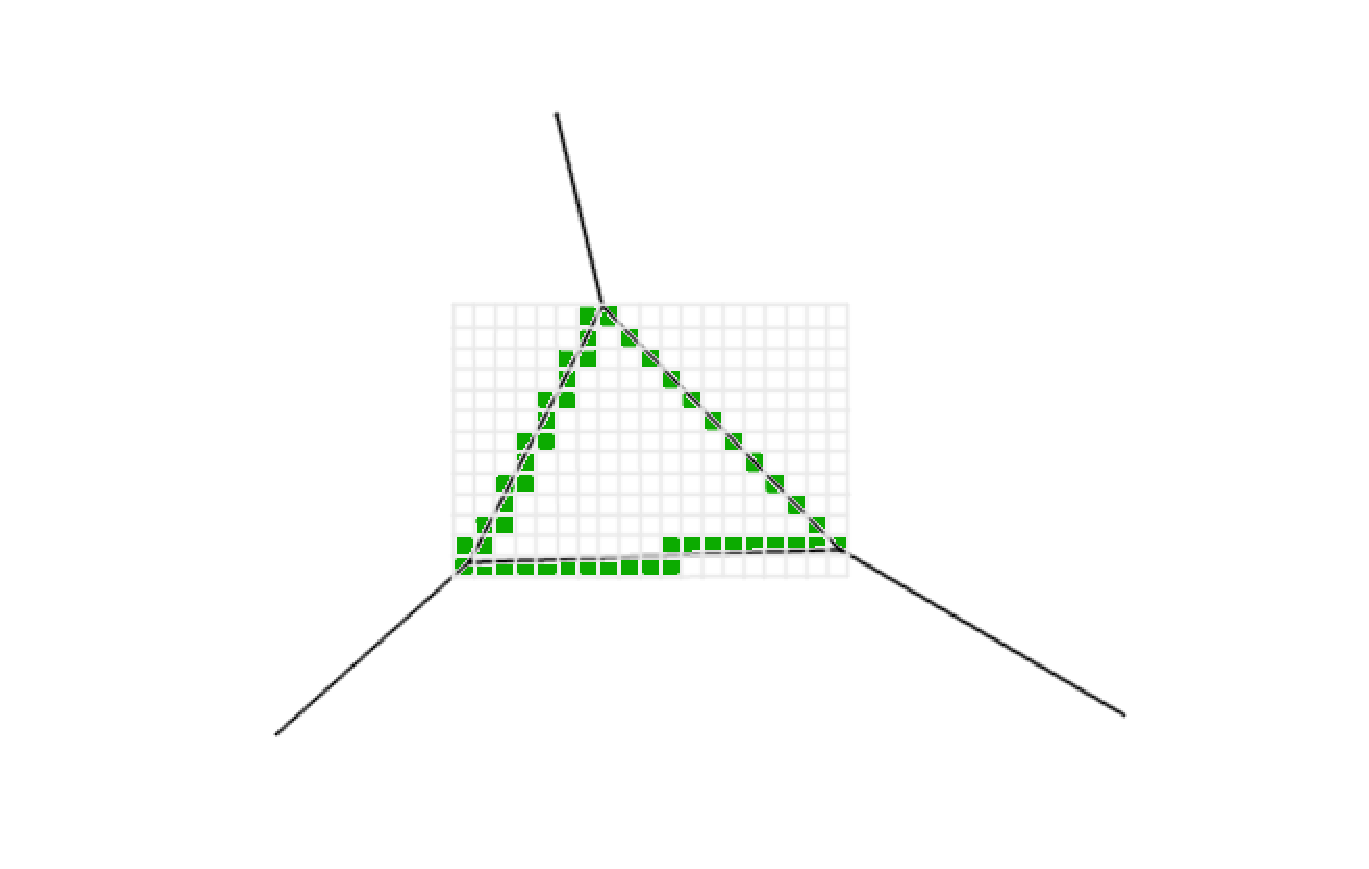
\includegraphics[scale=0.25]{../img/voxelize_2.eps}\\
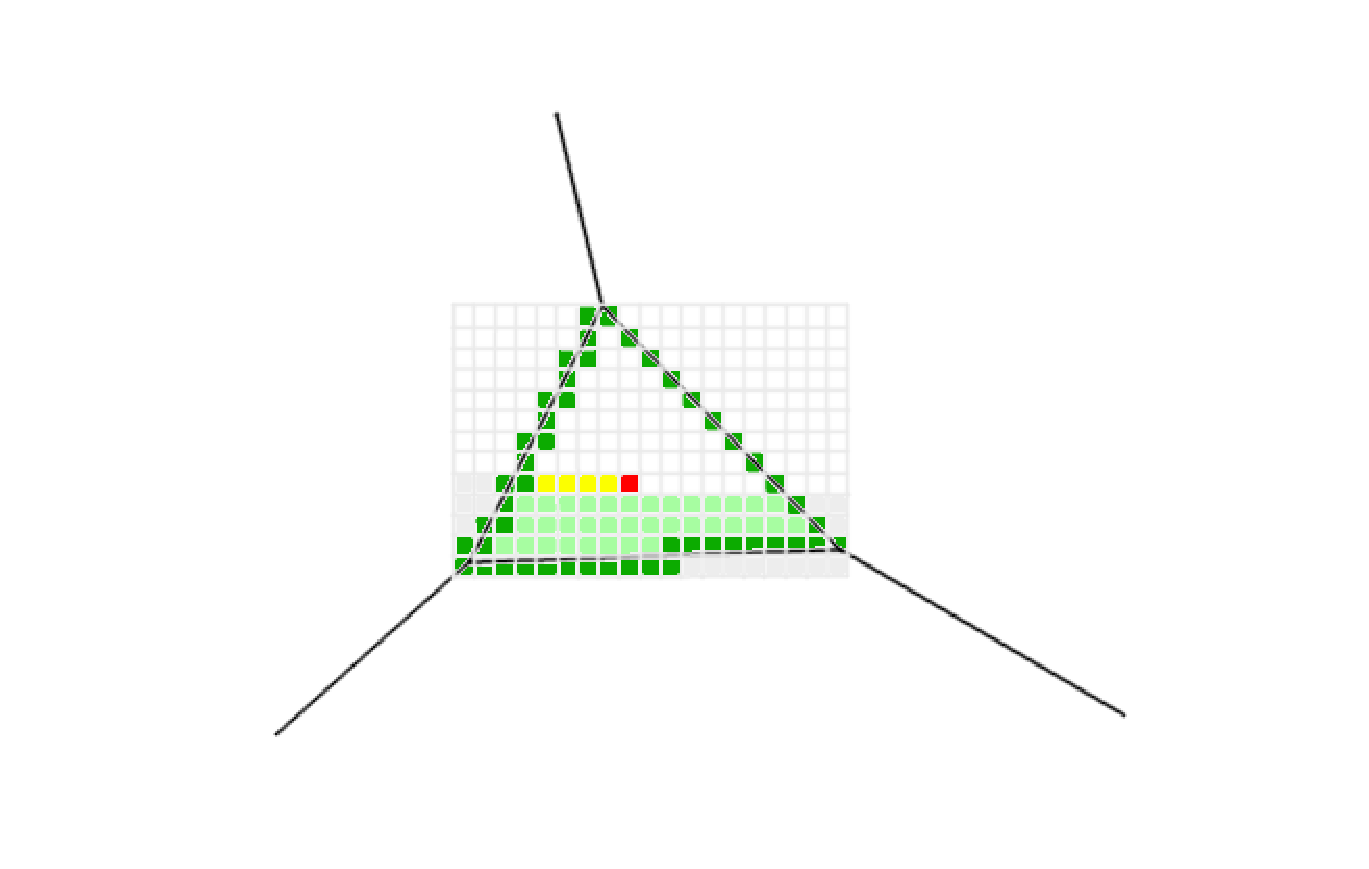
\includegraphics[scale=0.25]{../img/voxelize_3.eps}
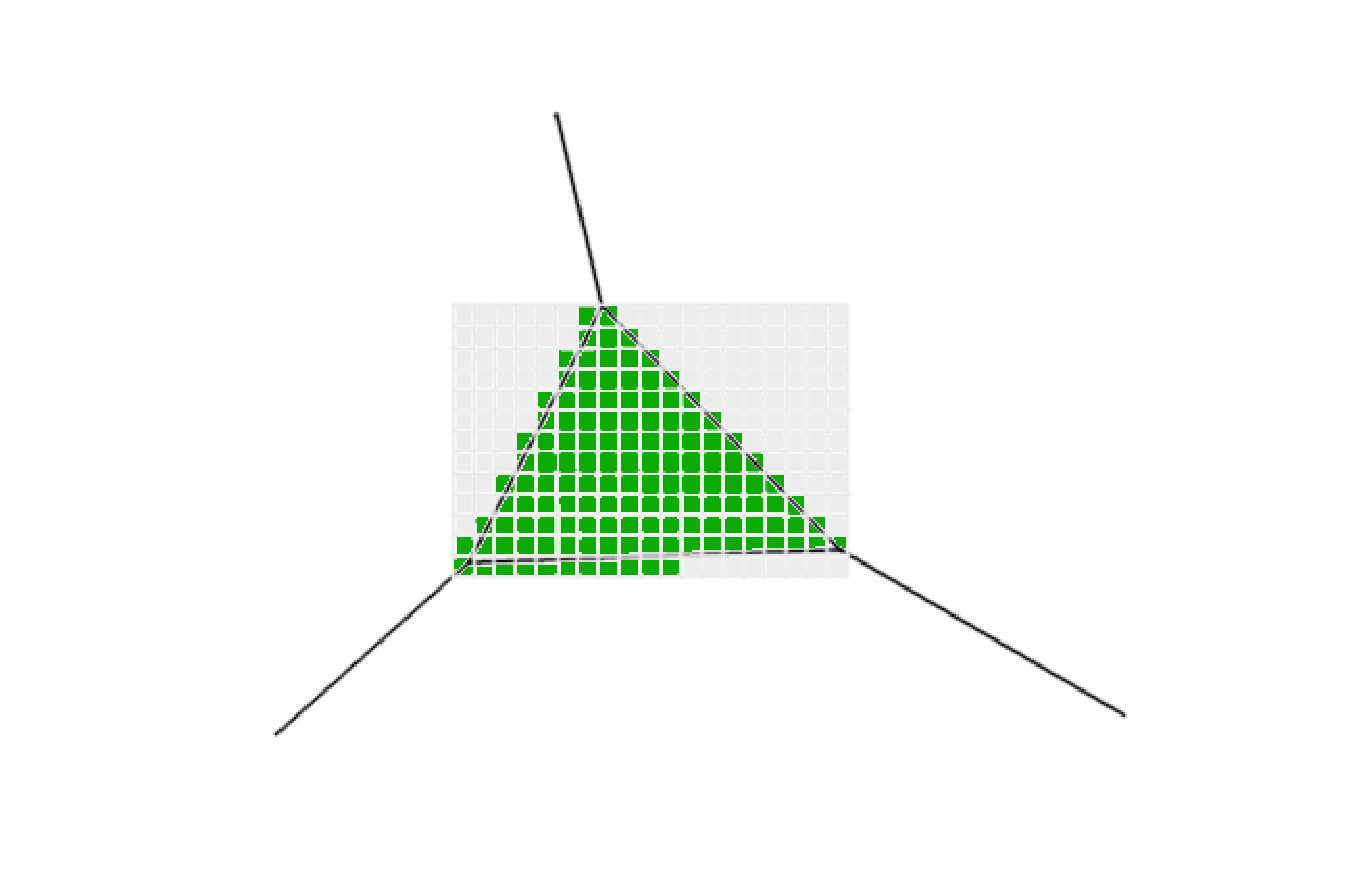
\includegraphics[scale=0.25]{../img/voxelize_4.eps}

\caption{Voxelization in step-by-step}
\label{fig:voxelize}

\end{figure}

\begin{itemize}
\item On the pre-computed minimum boundary rectangle start on the bottom and repeat for each line
\item in the line start from arbitrary side and process the elements consequently
\item After first crossing a rasterized edge start filling the elements (entry the face)
\item After second crossing a rasterized edge stop filling (leave the face).

\end{itemize}

In the second phase the algorithm fills the elements inside the object. The only problem is to
determine whether the given voxel is inside or outside the object. As described above, assumption of
starting with line outside the enclosed area gives us the right method. Also in this case the
bounding box will be needed. If the object cannot be wrapped the inside/outside property of element can 
not be determined.

\section{Editing functions}

Some functions are designed to changing size or shape of the object. Those functions are called 
\emph{editing function}.
During the editation of the object, user defines required values and the function deforms the
object properly. In case of the editing function \emph{scaling} for instance, a user defines the scaling
ratio.

\subsection{Truncate}

Truncate is the operation that affects a topology of mesh. From a given vertex it creates a new face with
surroundings of the original vertex. This is a common operation of mesh editation used e.g. in
3D editors.\\

\begin{figure}[ht]
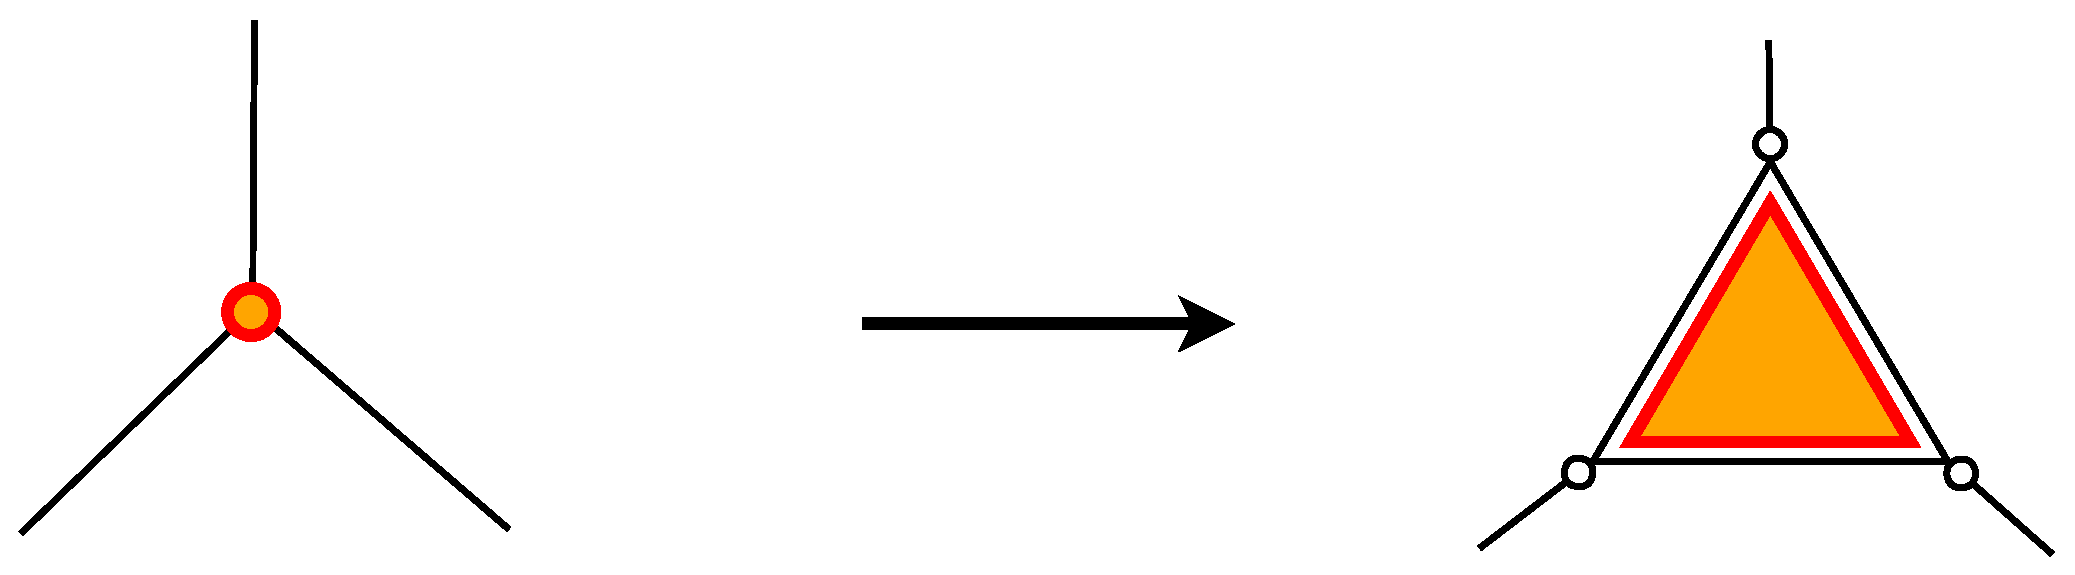
\includegraphics[scale=0.2]{../img/truncate.eps}
\caption{The red-marked vertex is a selected vertex to be truncated.
The face filled by orange color with red borders is the resulting face created by truncation}
\end{figure}

%This algorithm requires the capability of mesh to query the surrounding vertices of given vertex and
%adding the vertices and faces to the mesh.

\subsection{Bevel}

This operation is almost identical with \emph{truncation}. The only difference is the argument of the
operation. As the truncate operation creates a new face based on the given vertex, the bevel operation
creates the face from a given edge.\\

\begin{figure}[ht]
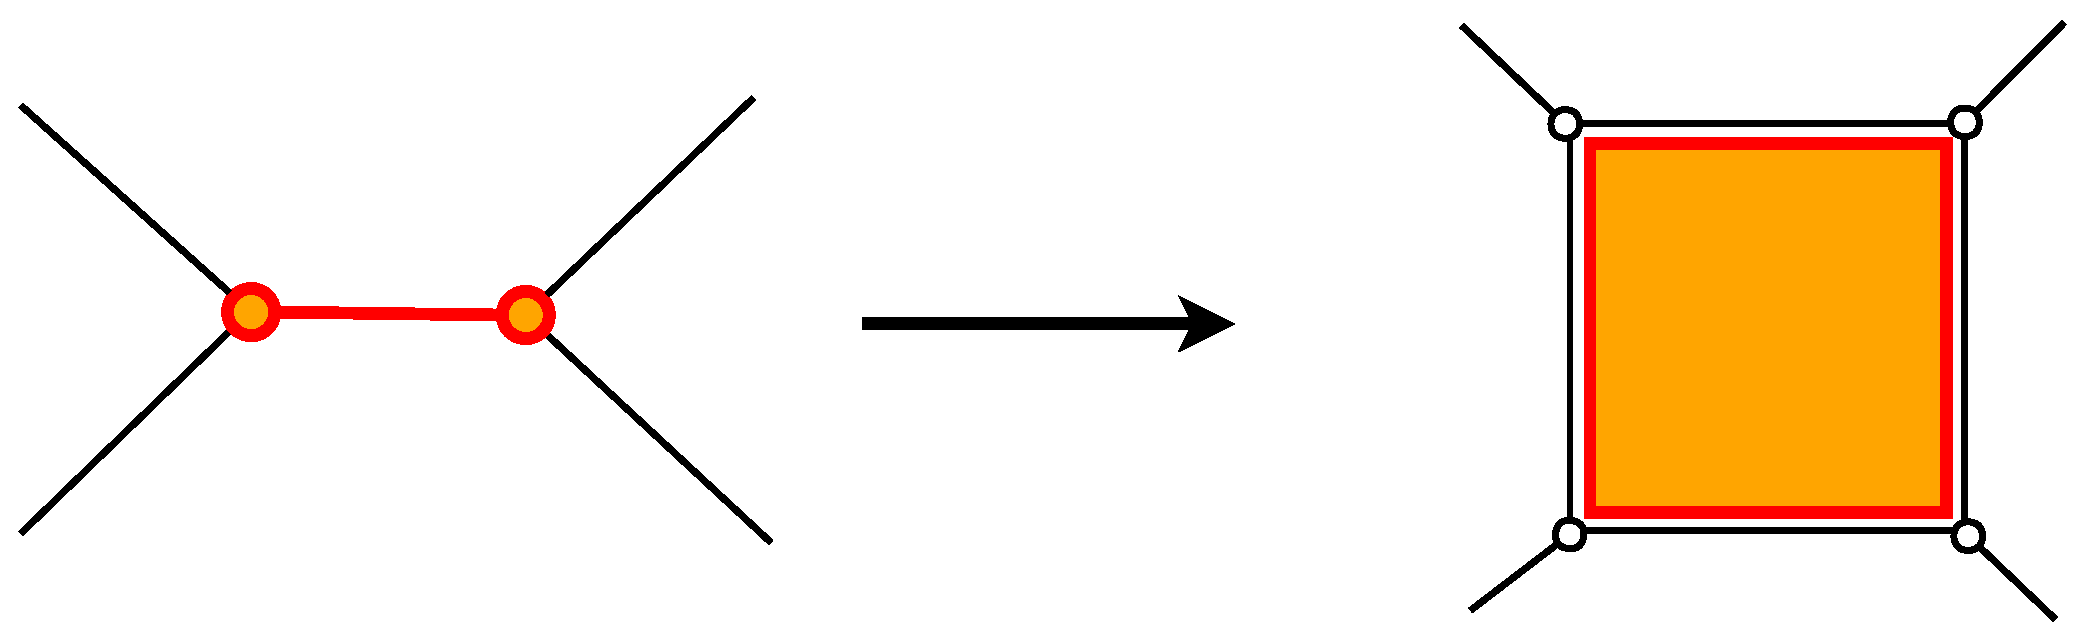
\includegraphics[scale=0.2]{../img/bevel.eps}
\caption{The red-marked edge is a selected edge to be beveled. As in the previous case, the resulting
face is filled by orange color.}
\end{figure}

%This algorithm has the same requirements as the truncate. In addition it requires the capability of
%querying to surrounding vertices of given edge.


\part{Analysis}
\chapter{Libraries}

What we did not yet mentioned is the implemented data structures that fulfills the described rules.
In this chapter there are introduced several libraries that are comonnly used. In following paragraphs
is shown the corelation with the structures shown in the previous chapter.

\section{OpenMesh}

\emph{OpenMesh}\cite{Botsch2002} is an open-source generic data structure for representing
and manipulating polygonal meshes. It is developed at the Computer Graphics Group, RWTH Aachen.
\\
\\
Restricting to the meshes introduced in chapter 2, OpenMesh is considered as a half-edge structure.
It is formed by kernel that set proper attributes such as triangular restriction or allowing to remove
vertices from mesh.
\\
To fully specify a mesh, several parameters can be given:\\

\textbf{Face type}: Specifies whether to use a general polygonal mesh or the triangle mesh.\\

\textbf{Kernel}: Stores the element of the mesh internally. User chooses from available
kernels according to expected usage. For example the decimation algorithm requires
efficient deletion/insertion thus the proper kernel for this case is kernel based on
linked list.\\

\textbf{Traits}: Traits is the class that enhances the mesh functionality such as
vertices removal or adding various attributes to elements.
\chapter{Designing the library}

There are a lot of libraries that offers the ability to represent the volume data
and the basic manipulation with it. There are also lot of published algorithms
that can be implemented.\\

Our goal is to create a generic set of algorithms that can be used on any implementation
of mesh that satisfies required concept. Before the algorithm is finally implemented,
we must completely describe the concept of the algorithm nor the behavior of algorithm
on specified mesh. The point of this goal is \emph{to think generally} regardless of
the specification of a potentionally used mesh.\\

\section{Observation}

Observing the algorithms step-by-step we can see that a single steps
of the algorithm are the variations of adding, removing and modifying the elements
of the mesh. In addition, the algorithms uses also a capabilities of querying
in mesh such as getting all adjancent vertices of given vertex or getting all
vertices in a container or any iterable structure.\\

Such a capabilities of the mesh are critical for implementing an algorithm.
The question then arises, ``Why do we implement the algorithms for meshes if
the usage of required operations might have suffice?" The answer can be relatively simple:
We are generally not able to determine how is a given structure controlled
without giving additional information.\\

Thus there is an option to build an algorithm working correctly over any structure
that fullfills the criteria that has been presented by the algorithm. Nowadays in C++,
we are able to build a template-based interface that modify a given structure according
to algorithm requirements during a compile time.\\

Before using this set of algorithms the user only defines a interface for chosen structure
and pass it as parameter.

\section{Concepts and algorithms}

Concept is specific according the requirements of an algorithm. Let us provide an example
algorithm and then we build a structure concept that requires the algorithm in order to work 
correctly.\\

\textbf{Example:}\\
The algorithm, that flips normal on each face of a given mesh.\\

\textbf{Solution:}\\
Before analyzing the algorithm, we can see that input is a mesh (not closely specified)
that returns modified mesh. The idea of the algorithm is simple; pick all faces
and flip the normal of each one. Obviously, the mesh is required to have a faces. This is not an
unnecessary point because there are several implementations of mesh without faces; e.g.
vertex-edge mesh. Finally, let us summarize what \emph{attributes} are required by the algorithm.

\begin{itemize}
\item faces of a mesh
%\item normal of a face
\end{itemize}

Now when we have the required attributes, we need to specify which \emph{operations} are required.

\begin{itemize}
\item flipping the normal of a face 
\item capabilty of applying the operation on each face
\end{itemize}

\textbf{Question:}\\
What if the structure does not have a method that flips the normal of a face?\\

After all, the algorithm can be build without providing a method that flips a normal;
it can flip the normal of a face by itself.
There are two possible approaches of solving this question. The first: create separately
next algorithm with different requirements. The second: build an \emph{adaptor} that
has the same functionality as required method that flips normals and use it as method
in the algorithm described above instead required method.\\

Both cases requires additional points of concept instead the ommited one.
In order to reverse the normal of a face manually, it is required:

\begin{itemize}
\item the normal of a face
\item getting the face normal
\item setting the face normal
\end{itemize}

It is up to us how we design the algorithms and the level of implementation. As more sophisticated
the adaptors are than more cases of mesh implementation can be covered. If the compiler does not
find the require methods and is able to build an adaptor then does not bother the user and build
a modified method. Naturally, adaptor may have own requirements therefore we can assume that
some point of concepts can be replaced with different ones.
\chapter{Algorithms Decomposition}

In this chapter are decomposed the algorithms (see chapter \ref{chap:op_al}) so that basic
operations over polygon
mesh can be summarized. The word ``\emph{basic}" is relative according the chosen level.
In this thesis is chosen such level that leads to the least count of operations in total.\\
\\
If the mesh does not fulfill the concept of the algorithm \emph{adaptors} can be used instead
of the absent operators. An adaptor behaves like an operator but in fact it is the algorithm that
makes a desired step as a result. In the other words it is the operator implemented in terms
brute-force. In some cases, lack of an operator can not be replaced by an adaptor.\\
\\
The algorithms described in this chapter are only the small part of all algorithms. The emphasized
algorithms are primarily the commonly used, the algorithms that changes the mesh topology and
the conversion algorithm between voxel and polygon mesh representation.

\section{Converting between representations}

\subsection{Marching cubes}

The algorithm has the specific requirements for the mesh and also for the voxel map (See algorithm
description \ref{sub:march}). However the voxel map can be in various forms some special cases
of marching cubes are explained.

\begin{algorithm}[H]
\caption{Marching cubes}
\label{alg:mc}
\begin{algorithmic}[1]
	\Function{Marching cubes}{$voxelMap$}
			\State $mesh$ := empty mesh

		\For{\textbf{each} $voxel$ \textbf{in} $voxelMap$}
			\State $cubeType$ := Determine Cube Type($voxel$)
			\State $faces$ := Create Faces($cubeType$)
			\For{\textbf{each} $face$ \textbf{in} $faces$}
				\State Add Face To Mesh($mesh$, $face$)
			\EndFor
		\EndFor
		\State \Return{$mesh$}
	\EndFunction
	\\
	\Function{Determine cube type}{$voxel$}
		\State $configuration$ := initial configuration
		\State \Comment{configuration contains all the information}
		\State \Comment{	about each corner of the cube}
		\State \Comment{initial configuration assumes that all corners are outside}
		\State $corners$ := Get Voxel Corners($voxel$)
		\For{\textbf{each} $corner$ \textbf{in} $corners$}
			\If {$corner$ is inside the surface}
				\State Set in configuration the $corner$ as inside
			\EndIf
		\EndFor
		\State \Return{$configuration$}
	\EndFunction
\end{algorithmic}
\end{algorithm}

%\caption{The simplified pseudo-code of the algorithm Marching cubes}


From the pseudocode \ref{alg:mc} we can conclude that the structures used as a parameters
are required to support operations used in the algorithm. Thus the concept of the algorithm
is designed as follows:

\begin{itemize}
\item $mesh$ is required to support $face$ structure \emph{(line 6)}
\item $mesh$ is required to support adding the $faces$ \emph{(line 7)}
\item $voxelMap$ is required to support $voxel$ structure \emph{(line 3)}
\item $voxelMap$ is required to support getting all the $voxels$ \emph{(line 3)}
\item $voxelMap$ is required to support getting all the $corners$ of each $voxel$ \emph{(line 18)}
\item $voxelMap$ and $mesh$ are required to have a $cubeType$ convertible to a set of $faces$ \emph{(line 5)}
\end{itemize}

\subsection{Voxelization}

Compared to the \emph{Marching cubes} algorithm, the requirements for the voxel map structure
are more comprehensive. As mentioned in description \ref{sub:vox}, the algorithm consequently rasterizes
the edges, the faces and finally fills the object.

\begin{algorithm}[H]
\caption{Voxelization}
\label{alg:vox}
\begin{algorithmic}[1]
	\Function{Voxelize mesh}{$mesh$}
			\State $voxelMap$ := map of empty voxels

		\For{\textbf{each} $face$ \textbf{in} $mesh$}
			\State Voxelize face($face$, $voxelMap$)
		\EndFor
		\State Run Floodfill($voxel map$)
		\State \Return{$voxel map$}
	\EndFunction
	\\
	\Function{Voxelize face}{$face$, $voxelMap$}
		\For{\textbf{each} $edge$ \textbf{in} $face$}
			\State Voxelize edge($edge$, $voxelMap$)
		\EndFor
		\State Run Face Floodfill($face$, $voxel map$)
		\State{\textbf{update} $voxelMap$}
	\EndFunction
	\\
	\Function{Voxelize edge}{$edge$, $voxelMap$}
		\State $v_{0}$ = First Vertex($edge$)
		\State $v_{1}$ = Second Vertex($edge$)
		\For{\textbf{each} $voxel$ \textbf{between} $v_{0}$ \textbf{and} $v_{1}$}
			\State Set As Filled($voxel$)
		\EndFor
		\State{\textbf{update} $voxelMap$}
	\EndFunction
\end{algorithmic}
\end{algorithm}
\chapter{Adapters}
\label{chap:adapter_analysis}

If the polygon mesh does not satisfy the designed concept of the algorithm then the compiler
raises an error. Nevertheless, in some cases, there is an option to create an additional function
that performs according the requirements for the absent operation.
In C++ standard library, adapters are used to build function objects out of ordinary
functions or class methods\cite{Simonis2000}.\\
\\
Inspired by the adapters from the C++ standard library, we create a set of adapters
for our generic algorithms library.
This chapter discribes the purpose of adapters in the implementation of generic algorithms
supported by several examples. It is primarily used in case of the absence of any required operation
used in algorithm.

\section{Observation}

Same as algorithms, adapters have specific requirements to be created. From this point of view,
we can state that an adapter has a capability to substitute a point of the concept with
the other ones that are required for the adapter.\\
\\
That statement is supported in following paragraphs.

\section{Get-Adjacent-Vertex-of-Vertex Adapter}

If the polygonal mesh is not in a representation that contains direct information about adjacency of two
vertices then the mesh can not effectively 
get the adjacent vertices from a given vertex. Obviously, no algorithm that contains query for
adjacent vertices of a vertex can be working over such a structure.\\
\\
However, using the brute-force, we can determine which ones from vertices are in adjacency with
the queried vertex. In the other words, demanded vertices can be acquired after checking all
faces that contain the queried vertex.

\subsection{Concept of the Adapter}

Assuming the structure is non-edge-based, we add an assumption that the structure is face-based
so it supports the face structure that provides information about contained vertices in the correct
order. The points of the concept are as follows:

\begin{itemize}
\item mesh is required to support getting all faces of the mesh
\item mesh is required to support getting all vertices of a face in the mesh
\end{itemize}
Finally, we can conclude that the point ``\emph{mesh is required to support getting all adjacent vertices
of a vertex in the mesh}" can be substituted by these two points in a concept of any 
algorithm. On the other hand, the complexity of the operation raises from 
$\mathcal{O}(V_{vertex})$ to $\mathcal{O}(F_{mesh})$ where the $F_{mesh}$ is the number of the
faces in total and $V_{vertex}$ is the expected count of the adjacent vertices.
\part{Implementation}
\chapter{Hmira Library}

The library is written in C++ using the standard \emph{C++11}\cite{Naugler2013}. However the features
for metaprogramming are not yet as advanced as the ones from \emph{Boost}\cite{Abrahams2004} we
use Boost library, especially Boost Metaprogramming Library\cite{bmpl}
and Boost Preprocessor Library\cite{bpl} for metaprogramming purposes.

\section{Designing the Concept}

The important part of the generic library is the concept - the set of requirements for a template
used as parameter. After the concept is satisfied, a code can be built.\\
\\
Concept consists of axioms and constraints\cite{Sutton2012}. Constraints are statically evaluable
predicates of the properties. Axioms are the requirements on the types that can not be statically
evaluated.

\section{C++11}

The standard \emph{C++11} comes with new features such as lambda functions, static assertions and other
features that help us to pre-evaluate available constants during the compile-time.\\
\\
C++11 contains the header \texttt{\textless type\_traits\textgreater} that defines
a series of classes to obtain information during the compile-time.

\section{Boost}

Boost has a metaprogramming framework \texttt{boost::mpl}\cite{bmpl}. During the compile-time, it is
capable of evaluation logical or arithmetical expressions. Combined with \texttt{std::enable\_if}
or static assertion it can determine which function will be compiled and which not.

\section{Threading Building Blocks}

The library \emph{Threading Building Blocks}\cite{Reinders2010}\cite{Pheatt2008}
is multiplatform C++ template library
for task parallelism made by Intel\textregistered. It uses C++ templates to eliminate the need to
create and manage threads. The Hmira library uses the Threading Building Blocks in algorithms
that have a section which can be done parallely; in the chapter \ref{chap:alg_decomp}, the
section which can be done paralelly is labeled with \textbf{parallel}. E.g.: the \textbf{parallel for}
does not necessarily mean that the block must be a parallel loop; it means that the block of code
provides an option being done parallelly.

% Ukázka použití některých konstrukcí LateXu (odkomentujte, chcete-li)
% %%% Ukázka použití některých konstrukcí LaTeXu

\subsection{Ukázka \LaTeX{}u}
\label{ssec:ukazka}

This short subsection serves as an~example of basic \LaTeX{} constructs,
which can be useful for writing a~thesis.

Let us start with lists:

\begin{itemize}
\item The logo of Matfyz is displayed in figure~\ref{fig:mff}.
\item This is subsection~\ref{ssec:ukazka}.
\item Citing literature~\cite{lamport94}.
\end{itemize}

Different kinds of dashes:
red-black (short),
pages 16--22 (middle),
$45-44$ (minus),
and this is --- as you could have expected --- a~sentence-level dash,
which is the longest.
(Note that we have follwed \verb|a| by a~tilde instead of a~space
to avoid line breaks at that place.)

\newtheorem{theorem}{Theorem}
\newtheorem*{define}{Definition}	% Definice nečíslujeme, proto "*"

\begin{define}
A~{\sl Tree} is a connected graph with no cycles.
\end{define}

\begin{theorem}
This theorem is false.
\end{theorem}

\begin{proof}
False theorems do not have proofs.
\end{proof}

\begin{figure}
	\centering
	
\includegraphics[width=30mm]{../img/logo.eps}
	\caption{Logo of MFF UK}
	\label{fig:mff}
\end{figure}


\chapter*{Conclusion}
\addcontentsline{toc}{chapter}{Conclusion}


%%% Seznam použité literatury
%%% Seznam použité literatury je zpracován podle platných standardů. Povinnou citační
%%% normou pro bakalářskou práci je ISO 690. Jména časopisů lze uvádět zkráceně, ale jen
%%% v kodifikované podobě. Všechny použité zdroje a prameny musí být řádně citovány.

%\begin{thebibliography}{99}
%
%\bibitem{lamport94}
%  {\sc Lamport,} Leslie.
%  \emph{\LaTeX: A Document Preparation System}.
%  2. vydání.
%  Massachusetts: Addison Wesley, 1994.
%  ISBN 0-201-52983-1.
%
%\end{thebibliography}

\bibliographystyle{ieeetr}
\bibliography{thesis_citations}
\addcontentsline{toc}{chapter}{\bibname}


%%% Tabulky v bakalářské práci, existují-li.
\chapwithtoc{List of Tables}

%%% Použité zkratky v bakalářské práci, existují-li, včetně jejich vysvětlení.
\chapwithtoc{List of Abbreviations}

%%% Přílohy k bakalářské práci, existují-li (různé dodatky jako výpisy programů,
%%% diagramy apod.). Každá příloha musí být alespoň jednou odkazována z vlastního
%%% textu práce. Přílohy se číslují.
\chapwithtoc{Attachments}

\openright
\end{document}
